\documentclass{scrartcl}
\usepackage[utf8]{inputenc}
\usepackage[german]{babel} 
\usepackage[colorlinks=true,
        linkcolor=black,
        citecolor=black,
        filecolor=black,
        urlcolor=black,
        bookmarks=true,
        bookmarksopen=true,
        bookmarksopenlevel=3,
        plainpages=false,
        pdfpagelabels=true]{hyperref}
\usepackage[square, numbers]{natbib}
\usepackage{setspace}
\usepackage[a4paper,left=2cm,right=2cm,top=2cm,bottom=4cm]{geometry}
\usepackage{graphicx}
\usepackage{morefloats}
\usepackage{ulem}
\usepackage{units}
\usepackage{wrapfig}
\usepackage{amsmath}
\usepackage{tikz}
\usepackage{colortbl} %Matze
\usepackage{xcolor}		%Matze 
\usepackage{pdfpages} %Matze
\usepackage{picinpar} %Matze
\definecolor{hellblau}{rgb}{0.8,0.8,1}
\definecolor {hellgruen}{rgb}{0.5,1,0.8}
%\usepackage{minted}
\usepackage[section]{placeins}
\usepackage{listingsutf8}
%\usepackage{wrapfig}
%\usepackage{pdfpages}
%\nocite{*}

\lstdefinestyle{customc}{
  belowcaptionskip=1\baselineskip,
  breaklines=true,
  frame=L,
  xleftmargin=\parindent,
  language=C,
  showstringspaces=false,
  basicstyle=\footnotesize\ttfamily,
  keywordstyle=\bfseries\color{green!40!black},
  commentstyle=\itshape\color{purple!40!black},
  identifierstyle=\color{blue},
  stringstyle=\color{orange},
}

\lstset{escapechar=@,style=customc, extendedchars=\true,
    inputencoding=utf8/latin1}

\parindent0mm

\newcommand {\Ohm} {$\Omega\ $}

\bibliographystyle{alphadin}

\begin{document}
\title{Projektarbeit 'Bauteileautomat'}
\author{
	Jan Krüger  \\
	Friedrichstraße 24 \\
	75417 Mühlacker \\
	Mtkl Nr: 37032 \\
	\and 
	Gregor Süß \\
	August-Dürr Straße 9 \\
	76133 Karlsruhe \\
	Mtkl Nr: 36496 \\
	\and
	Matthias Weißhaar \\
	Strümpfelbacher Straße 184\\
	71384 Weinstadt\\
	Mtkl Nr: 30250\\
	}

\date{\today}

\maketitle
\newpage

\tableofcontents
\newpage
\onehalfspace
\section{Einführung}
\subsection{Aufgabenstellung}
Für die Bereitstellung von elektronischen Bauteilen für die Studierenden der Elektrotechnik ist ein Ausgabeautomat zu entwickelen und zu erstellen. Der Automat ermöglicht den Studenten der Fakultät EIT zu jeder Tageszeit den Zugriff auf Elektronikbauteile (für ihre Studienprojekte und für den privaten Gebrauch). Der Automat soll viele kleine Fächer enthalten, damit aus einem reichhaltigen Sortiment an Bauteilen ausgewählt werden kann. Die Auswahl der Bauteile kann am Automaten oder vorab per Intranet erfolgen. Vor der Ausgabe der Teile ist eine Authentifizierung mit dem Studentenausweis am Automaten erforderlich. Der Bauteilebestand und die Verrechnung der entnommenen Bauteile sollen über eine Datenbank protokolliert werden. 

\subsection{Einleitung}
Der (Zeit-)Aufwand, der für die Erfüllung der Aufgabenstellung erforderlich ist, übersteigt das zeitliche Pensum einer Projektarbeit um ein vielfaches. Daher wurde die Aufgabenstellung in einer Gruppe bearbeitet und in drei Teile aufgeteilt. Ein besonderes Augenmerk lag auf einer klaren Trennung der Bereiche, damit eine enge Zusammenarbeit zwischen den Gruppenmitgliedern erreicht werden konnte. Im Hinblick auf die Ziele der Projektarbeit
(Projektgruppen die voneinander abhängig sind, Arbeiten nach Pflichten- und Lastenheften, etc) erschien diese Vorgehensweise als die beste. Der Aufbau dieses Dokuments spiegelt die klare Trennung der Aufgabenbereiche wider. Es ist in die drei Bereiche Elektronik, Software und Mechanik gegliedert, die erst einmal für sich selbst stehen und zusammen die Gesamtheit der Projektarbeit darstellen. Ziel dieses Dokuments ist es, die Arbeit zu dokumentieren und dem Leser einen Ansatzpunkt zur Weiterentwicklung des Automaten zu geben. 

\subsection{Aufgabenverteilung}
\begin{itemize}
\item
Jan Krüger betreut den Bereich 'Elektronik'. Dieser Bereich beinhaltet die Konzeption, Entwicklung und den Aufbau der Steuerplatine, der Verkabelung des Automaten und das Testen der Komponenten. Weiterhin gehört die Absprache der Bedürfnisse für den mechanischen Aufbau mit dem Bereich 'Software' zu seinem Aufgabengebiet. 
\item
Gregor Süß betreut den Bereich 'Software'. Er ist zuständig für die Konzeptionierung und Programmierung des Automaten. 
\item
Matthias Weißhaar betreut den Bereich 'Mechanik'. Dieser Bereich beinhaltet die Konzeption, Entwicklung und den Aufbau der mechanischen Komponenten, wie auch den Funktionstest derselben. 
\end{itemize}



\newpage

\section{Mechanik}
\label{Mechanik}
Dieses Kapitel dokumentiert die mechanische Funktionsweise und die Berechnung der zugehörigen Komponenten. Der Automat soll ca. 1000 Boxen enthalten, um eine große Auswahl zu gewährleisten. Damit dies in einer kompakten Bauweise möglich ist, werden drei unterschiedlich große Boxen verwendet. Die Boxen befinden sich in verschiedenen Schächten. 
Ein Schacht besteht aus jeweils zwei L-Profilen, die mit Schrauben an den Aluminiumprofilen der Rückwand befestigt werden. Die Größe der Schächte ist jederzeit änderbar und somit für jede Boxengröße variabel einstellbar. Ein Greifer, der auf X-Y-Z-Achsen verschiebar ist, fährt den ausgewählten Schacht an und greift anschließend die entsprechende Box. An der Seite des Automaten ist ein Rutsche angebracht, die zur Ausgabe der Teile dient. Der Greifer fährt diese an und kann durch ein Drehgelenk die Box um $180^\circ$ drehen und das gewünschte Teil auswerfen.


\subsection{Greifer}

\subsubsection{Anforderungen}


Der Greifer hat den sicheren Transport der Boxen zwischen den Schächten und der Rutsche zu gewährleisten. Er muss ein Drehgelenk beinhalten, das sich um $180^\circ$ drehen lässt. Weiter sind vom Greifer zwei verschieden große Boxen mit einem maximalen Gewicht von 1000g zu befördern. Damit die Ausgabe der Teile nicht zu lange dauert, muss die Geschwindigkeit des Greifvorgangs entsprechend hoch sein.


\subsubsection{Realisierung des Greifers}

Der Greifmechanismus erfolgt über zwei 20cm lange Greifarme aus Aluminium, wobei ein Greifarm fest verbaut ist und der andere über eine Trapezgewindespindel verfahrbar ist. Für den Antrieb der Spindel werden zwei Zahnräder verwendet, welche mit einem Schrittmotor verbunden sind. Damit der bewegliche Greifarm nicht verkantet, wird er über eine zusätzliche Welle geführt. Moosgummi auf dem Greifarm erhöht die Haftkraft zwischen den Boxen und den Greifarmen. Der Drehmechanismus erfolgt ebenfalls über zwei Zahnräder und einen Schrittmotor. Ein Zahnrad ist auf einer Welle befestigt, die auf einer Seite fest mit dem Greifer verbunden ist und auf der anderen Seite in einem Rillenkugellager gelagert ist. Durch das zweite Zahnrad, das durch einen Schrittmotor angetrieben ist, kann die Welle  mit dem Greifer rotiert werden. 


\subsubsection{Antrieb}

Alle relevanten Eigenschaften(Presskraft, Verfahrensgeschwindigkeit und Schrittlänge) sind abhängig vom Schrittmotor 
des Greifmechanismus. Für die richtige Dimensionierung des Schrittmotors sind entsprechende Berechnungen erforderlich.

\begin{itemize}

\item Haltekraft des Greifarms

Das Drehmoment des Motors muss den sicheren Transport einer Box mit einem Gewicht von 1000g gewährleisten. Zur Berechnung des Drehmoments wird die Presskraft benötigt, die der dynamische Greifarm auf die Box ausübt. Hier handelt es sich um einen Erfahrungswert, da verschiedene Berechnungsvariablen (z.b. Reibunkskoeffizent von Polystrol und Moosgummi) nicht vorhanden sind. Der Wert wurde daher auf $F=50N$ ausgelegt und bewußt höher gewählt, damit die Boxen auch bei kleinen Stößen und Vibrationen nicht aus dem Greifarmen rutschen können.\\
\newline

Durch die Umwandlung von einer Drehbewegung in eine Längsbewegung entsteht ein Wirkungsgrad, welcher durch den 
Steigungswinkel des Trapezgewindes und den Gewindereibungswinkel berechnet werden kann.\\

Den Steigungswinkel erhält man durch:

\[tan(\alpha)=\dfrac{P}{d\cdot \pi}=\dfrac{20mm}{4mm\cdot \pi}=\dfrac{5}{\pi}\]

\begin{tabbing}
mit \= P: Spindelsteigung\\
    \> d: Spindelnenndurchmesser  \\
		\> $\alpha$: Steigungswinkel\\
\end{tabbing}

Für ISO-Trapezgewinde mit geschmierter Mutter und einem Reibwert von $\mu=0.04$ erhält man den Gewindereibungswinkel mit:

\[ \rho=\mu\cdot 1.07= 0.04\cdot 1.07=0.043 \]

\begin{tabbing}
mit \= $\rho$: Gewindereibungswinkel\\
    \> $\mu$: Reibwert  \\
\end{tabbing}

Mit dem Steigungswinkel und dem Gewindereibungswinkel kann nun der Wirkungsgrad berechnet werden:

\[\eta=\dfrac{tan(\alpha)}{tan(\alpha +\rho)}=\dfrac{tan(\dfrac{5}{\pi})}{tan(\dfrac{5}{\pi}+0.043)}=3.08\]

\begin{tabbing}
mit \= $\eta$: Wirkunsgrad \\
\end{tabbing}

Das Antriebsdrehmoment der Spindel ergibt sich aus der Presskraft, der Steigung und dem Wirkungsgrad des Trapezgewindes: \\

\[M=\frac{F\cdot P}{1000\cdot 2\pi \cdot \eta}=\frac{50N\cdot 4mm}{1000\cdot 2\pi \cdot 3.08}=0.01Nm\]
\newline

\begin{tabbing}
mit \= M: Antriebsmoment\\
    \> F: Presskraft \\
\end{tabbing}


Auf das Ergebnis müssen die Verluste durch die Lagerung und der Wirkungsgrad der Übersetzung aufgeschlagen werden. Zur Berücksichtigung  dieser Verluste sollte die ausgewählte Leistung des Antriebs um 60\% bis 100\% über dem errechneten Wert liegen.\\

Mit dem Übersetzungsverhältnis der Zahnräder und den Verlusten des Greifmechanismus erhält man das geforderte Drehmoment des Motors durch:

Übersetzungsverhältnis der Zähnrräder:\\
\[i=\frac{z_2}{z_1}=\frac{30}{60}=0.5\]	

das Antriebsmoment des Schrittmotors:\\		
		
\[M_{Motor}=M_{Spindel}\cdot i \cdot R=0.01Nm \cdot 0.5 \cdot 1.6= 8Nmm \]

\begin{tabbing}
mit \= i: Übersetzungsverhältnis\\
    \> R: Reibungsverluste \\
\end{tabbing}






\item Schrittlänge

Die Schrittlänge ist der kleinstmögliche Weg, den der Greifarm zurücklegen kann. Bei einem Schritt des Motors wird dieser Weg zurückgelegt. Alle anderen Wege ergeben sich als ein vielfaches der Schrittlänge. Das weiche Moosgummi auf den Greifarmen und die Elastizität der Boxen erfordern eine feine Abstimmung der Presskraft der Greifarme. Für eine anwendungsgerechte Einstellung ist eine kleine Schrittlänge erforderlich.
\newpage



Mit dem Übersetzungsverhältnis kann die Schrittlänge des Greifers berechnet werden:
\[S=\frac{P}{\frac{360^\circ}{\alpha}}\cdot i=\frac{4mm}{\frac{360^\circ}{1.8^\circ}}\cdot 0.5=0.01mm\]


\begin{tabbing}
mit \= $\alpha$: Schrittwinkel des Elektromotors\\
    \> P: Steigung der Trapezgewindespindel
\end{tabbing}

Die geringe Schrittlänge ist ausreichend um die benötigte Presskraft einzustellen. Toleranzen des Gewindes oder der Schritte des Schrittmotors können vernachlässigt werden.
\newline

 
\item Geschwindigkeit des Greifarms\\

Um einen Schacht anzufahren müssen die Greifarme schon in der richtigen Schachtgröße positioniert werden. 
Die Positionierung findet während der Anfahrt an die jeweiligen Schächte statt. Somit muss nur noch das tatsächliche Greifen in einem gesonderten Arbeitsgang stattfinden. Hier ist der Verfahrensweg so klein $s<5mm$, dass die Geschwindigkeit größtenteils irrelevant ist. 

\end{itemize}



\subsubsection{Kugellager}

Um das Kugellager richtig zu wählen und eine lange Lebensdauer zu garantieren, wird die nominelle Lebensdauer nach 
ISO 281 berechnet:\\

\[L_{10h}=(\frac{C}{P})^p=(\frac{627N}{10N})^3 = 246492\]	


\begin{tabbing}
mit \= p: Lebensdauerexponent (bei Kugellager p=3)\\
    \> C: Dynamische Tragzahl in Kn(aus Lagertabelle des Herstellers) \\
    \> P: Dynamische äquivalente Belastung\\
		\> $L_{10}$: Lebensdauer in Millionen Umdrehungen bei 10\% Ausfallwahrscheinlichkeit
\end{tabbing}


Die nominelle Lebensdauer gibt an, wieviele Umdrehungen $90\%$ der Lager erreichen oder überschreiten bis die ersten Anzeichen von Werkstoffermüdung auftreten. Mit mehreren Millionen Umdrehungen bei 10\% Ausfallwahrscheinlichkeit ist für unsere Lager eine hohe Lebensdauer zuerwarten. Das Lager darf nicht zu groß dimensioniert werden, da ansonsten die Belastung der Lager zu gering wäre und kein Rollen der Wälzlager sondern Gleiten stattfindet. Gleitreibung sorgt für höheren Verschleiß und verkürzt daher die Lebensdauer.\\

Eine Lebensdauerberechnung ist für unsere Anwendung überflüssig, da die Kugellager nur sehr kleine Kräfte aufnehmen.
Zur Vervollständigung wurde diese jedoch trotzdem durchgeführt.



\subsubsection{Antrieb und Übersetzung Drehgelenk}

Das Drehgelenk wird ebenfalls über einen Schrittmotor angetrieben. Da hier nur eine Drehung von $180^\circ$ verlangt wird und der Motor ein hohes Drehmoment benötigt, wurde bei den Zahnrädern eine Übersetzung eingebaut.\\


Übersetzungsverhältnis der Zähnrräder:
\[i=\frac{z_2}{z_1}=\frac{14}{70}=0.2\]	

\begin{tabbing}
mit \= $z_1$: Zähnezahl\textsubscript{1} \\
    \> $z_2$: Zähnezahl\textsubscript{2} \\
\end{tabbing}

Durch das Übersetzungsverhältnis von 0.2 kann nun ein kleinerer Schrittmotor verwendet werden, dieser benötigt jedoch für eine Umdrehung die 5-fache Schrittanzahl. Auch hier müssen wieder Verluste eingerechnet werden und der Motor muss entsprechend größer dimensioniert werden.\\


Das Drehmoment berechnet sich zu:

\[M=F\cdot s\cdot i\cdot R = 10N\cdot  70mm\cdot 0.2\cdot 1.6 = 22.4Ncm\]

\begin{tabbing}
mit \= i: Übersetzungsverhältnis\\
    \> R: Reibungsverluste \\
		\> s: Länge(Kugellager-Greiferarm)\\
		\> F: Gewichtskraft des Greifers\\
\end{tabbing}





\subsubsection{Kugellager Drehgelenk}

Für die Ausgabe eines Bauteils rotiert das Kugellager $180^\circ$ und anschließend wieder $180^\circ$ zurück. Da nur eine Umdrehung pro Ausgabe am Kugellager notwendig ist, muss keine nominelle Lebensdauer für das Kugellager ausgerechnet werden. Es ist trotzdem wichtig, dass unser Kugellager mit einer mittleren Belastung betrieben wird. Das Verhältnis von dynamischer Tragzahl zu dynamischer äquivalenter Belastung sollte somit zwischen 8 und 15 liegen. Das Kugellager wird durch das komplette Gewicht von Greifer und Box radial belastet, welches mit 5kg ausgelegt wird. Eine axiale Belastung erfährt der Greifer nur durch die Beschleunigung der Z-Achse, welche hier gering ausfällt und somit vernachlässigt werden kann. 

 


 

\subsection{Achsen}

\subsubsection{Anforderungen X-Y-Z-Achse}

Um eine hohe Auswahlmöglichkeit im Automaten zu erreichen, muss dieser möglichst viele Boxen enthalten. Deshalb ist die größtmögliche Anzahl an Schächten im Automaten unterzubringen. Die L-Profile, welche die Schächte bilden, müssen sehr eng aneinander gereiht werden. Das Spiel zwischen den Schächten ist somit sehr gering und die Achsen müssen die jeweiligen Schächte präzise anfahren. \\
Die Ausgabezeit des Produktes ist für den Kunden wichtig und muss berücksichtigt werden. Damit der Kunde nicht zu lange auf sein gekauftes Bauteil warten muss, sind Verfahrensgeschwindigkeit und Beschleunigung der Achsen ebenfalls zu berücksichtigen und richtig zu dimensionieren. \\
Die Achsen müssen platzsparend im Automaten untergebracht werden und dürfen die Maße des Automaten nicht unnötig
vergrößern. Da die Verfahrenswege der Achse unterschiedlich lang sind, müssen die Berechnungen einzeln stattfinden. 
Der Automat soll eine lange Lebensdauer erreichen.\\



\subsubsection{Realisierung der Achsen}




Für den Vorschub der Achsen wurden Kugelumlaufspindeln verwendet, die jeweils mit zwei Linearführungen ein 
Linearmodul bilden. Die zwei Profilschienenführungen tragen die Masse des Greifmechanismus und garantieren die Einhaltung der linearen Bewegungsrichtung. Die Kugelumlaufspindel hat eine geringe Schrittlänge, welche sich im $\mu m$ Bereich einreiht, was für den Bauteileautomat ausreichend ist. Durch die geringe Reibung der Kugelumlaufspindel wird ein hoher Wirkungsgrad der Motoren und geringer Verschleiß erreicht, was zu einer hohen Lebensdauer der Achsen führt. Die Positioniergenauigkeit der Kugelumlaufspindel ist hoch und entspricht den Anforderungen unseres Automaten.\\


\begin{figure}[htbp] 
  \centering
     \includegraphics[width=0.8\textwidth]{Bilder/Z_Achse.jpg}
			\caption{Z-Achse}
  \label{fig:Bild1}
\end{figure}


Der Antrieb der Achsen erfolgt über einen Schrittmotor, welcher über eine Oldham-Kupplung mit der Welle verbunden ist.
Die Kupplung überträgt das Drehmoment des Motors an die Welle und kann geringe parallele Versätze ausgleichen, die durch Fertigungsfehler entstehen können.\\




\subsubsection{Antriebsmoment der Z-Achse}

Die Bewegung der Z-Achse muss, wie der Greifmechanismus, getrennt von den anderen Bewegungen stattfinden. Die Beschleunigung und Verfahrensgeschwindigkeit darf daher nicht zu gering ausfallen. Trotz Reibung und Wirkungsgrad der Kugelumlaufspindel muss das Antriebsmoment des Schrittmotors so gewählt werden, dass eine akzeptable Verfahrenszeit erreicht werden kann.


\begin{itemize}

\item \textbf{Reibungskraft}

Die Reibungskraft, die in den Linearführungen auftritt, kann mit der folgenden Formel berechnet werden:

\[F_R=\mu\cdot m\cdot g+f=0.003 \cdot 5kg \cdot 9.81\dfrac{m}{s^2}+5N = 0.1N + 5N = 5.1N\]

\begin{tabbing}
mit \=$\mu$: Dynamischer Reibungskoeffizent\\
		\>m: Masse des Greifers\\
		\>g: Erdbeschleunigung\\
		\>f: Dichtungsbeständigkeit\\
\end{tabbing}

Aus der Rechnung ist ersichtlich, dass die Masse des Greifers kaum eine Rolle auf die Reibungskraft hat. 
Der Großteil der Reibung entsteht durch die verschiedenen Dichtungselemente der Linearführung (z.b. Dichtungslippe), 
welche nicht von der Last abhängig sind.


\item \textbf{Beschleunigung}
 
Der maximal verfahrbare Weg der Z-Achse beträgt $s=186mm$. Die Hälfte dieses Weges soll in einer Zeit von maximal $t=3s$ zurückgelegt werden. Somit ist auch gegeben, dass die Z-Achse auf der anderen Hälfte wieder gebremst werden kann. 


\begin{tabbing}
Beschleunigung: \qquad \=$\ddot{x}_a=a$\\
Geschwindigkeit: 							\>$\dot{x}_v=a\cdot t$\\
Verfahrensweg:												\>$x_s=0.5\cdot a\cdot t^2$\\
\end{tabbing}

Aus dem Verfahrensweg und der Zeit ergibt sich eine konstante Beschleunigung von:

\[a=\dfrac{2\cdot s}{t^2}=\dfrac{2\cdot 93mm}{9s^2}= 21\dfrac{mm}{s^2}\]

Die notwendige Kraft für die Beschleunigung erhält man aus der Masse des Greifers:

\[F_a=m\cdot a=5kg \cdot 0.021\dfrac{m}{s^2}=0.11N\]

\item \textbf{Antriebsmoment}


Mit der Reibungskraft, der notwendigen Kraft für die Beschleunigung und einem Wirkungsgrad von $\eta=0.9$ der Kugelumlaufspindel kann nun das erforderliche Antriebsmoment berechnet werden: 

\[M=\dfrac{(F_R + F_a) \cdot P}{2\pi \cdot \eta}=\dfrac{(5.1N+0.11N)\cdot 4mm}{2\pi \cdot 0.9}= 3.69Nmm\]

\begin{tabbing}
mit \=$F_R$: Reibungskraft\\
		\>$F_a$: Kraft für Beschleunigung\\
		\>P: Steigung Kugelumlaufspindel\\
		\>$\eta$: Wirkungsgrad Kugelumlaufspindel\\
		
\end{tabbing}

Auch hier müssen noch die Verluste durch die Lagerung der Kugelumlaufspindel hinzugerechnet werden. Zusätlich sollte noch 
eine Sicherheit mit eingerechnet werden. Insgesamt sollte das Antriebsmoment um das 1.5fache erhöht werden.

\[M_{Schrittmotor}=M \cdot 1.5 = 3.69Nmm \cdot 1.5 = 5.54Nmm\]

		
Der gewählte Schrittmotor muss somit ein Drehmoment von mindestens $M_{Schrittmotor} = 5.5Nmm$ aufweisen.


\end{itemize}


\newpage

\subsubsection{Linearführung Z-Achse}

\begin{itemize}








 
\begin{figure}[htbp]
	% minipage mit (Blind-)Text
	\hspace{10mm}
	\begin{minipage}[c]{0.5\textwidth} 
	
	
\item \textbf{Momente$(M_A/M_B/M_C)$}	\\
\newline
Die zulässigen statischen Momente der Linearführungen dürfen nicht überschritten werden, damit ein sauberer Lauf und eine lange Lebensdauer garantiert wird. Zudem wird eine Sicherheit von 3 eingebaut, damit Mehrbelastungen durch
dynamische Bewegungen nicht zu einer Überlast führen. Die statischen Momente $M_B$ und $M_C$ sind nicht vorhanden oder sehr gering und können vernachlässigt werden. Das kritische Moment $M_A$ ergibt sich durch die Gewichtskraft des Greifers und der Länge des Greifers. Das Moment wird auf zwei Linearführungen aufgeteilt und muss eine Sicherheit beinhalten.
	% \caption{Der Text}
	% \label{Text}
	\end{minipage}
	% Auffüllen des Zwischenraums
	\hfill
	% minipage mit Grafik
	\begin{minipage}[c]{0.4\textwidth}
	% \textwidth bezieht sich nun auf die Minipage
	\includegraphics[width=\textwidth]{Bilder/Momente.jpg}
	\caption{Momente}
	\end{minipage}

\end{figure}


\[M_A>\dfrac{m\cdot g \cdot l \cdot s}{2}=\dfrac{5kg\cdot 9.81\dfrac{m}{s^2}\cdot 0.1m\cdot 3}{2}=7.5Nm\]


\begin{tabbing}
mit \=m: Masse\\
		\>g: Erdbeschleunigung\\
		\>l: Länge\\
		\>s: Sicherheit\\
\end{tabbing}


Das zulässige statische Moment der beiden Linearführungen muss mindesten 7.5Nm betragen.\\



\item \textbf{Nennnutzungsdauer}

Die Nennnutzungsdauer gibt den Verfahrensweg an, den $90\%$ der Linearführungen desselben Typs unter identischen 
Bedingungen zurücklegen können ohne dabei Schäden zu erleiden. Die Linearführungen des Bauteileautomats werden unter 
fast perfekten Bedingungen betrieben (kein Schmutz, keine hohen Temperaturen, niedrige Last). Der Anspruch der Lebensdauer für den Bauteileautomat wird damit weit übertroffen und eine Berechnung wird überflüssig. Dies gilt auch für die X-Y-Achsen.
\newline



%BERECHNUNG NICHT NOTWENDI
%\[P=F + \dfrac{C_0}{M_C}\times (F \times L_r) + \dfrac{C_0}{M_A}\times (F\times L_p)\]

%\begin{tabbing}
%mit \=F: Gewichtskraft des Greifers\\
%		\>$C_0$: Statische Tragzahl\\
%		\>$M_A$: Zulässiges statisches Moment - Steigungsrichtung  \\
%		\>$M_C$: Zulässiges statisches Moment - Rollrichtung\\
%		\>$L_p$: Distanz (Führungswagen-Lasmittelpunkt in Steigungsrichtung)\\
%		\>$L_r$: Distanz (Führungswagen-Lasmittelpunkt in Rollrichtung)\\
		
%\end{tabbing}

%\[L=(\dfrac{C}{P})^3\cdot50=(\dfrac{5kN}{P})^3\cdot50\]

%\begin{tabbing}
%mit \=L: Nennnutzungsdauer\\
%		\>P: Nutzlast\\
%		\>C: Dynamische Tragzahl\\
		
		
%\end{tabbing}


\end {itemize}






\subsubsection{Kugelumlaufspindel der Z-Achse}


\begin{itemize}

\item \textbf{Zulässige Axiallast}
 
Eine Berechnung der zulässigen Axiallast ist für die X-Z-Achsen nicht notwendig. Die Axialkräfte (Beschleunigungskraft) sind zu gering, um die zulässige Axiallast zu überschreiten. 



%BERECHNUNG BEI DER Z_ACHSE nicht nötig
%\item \textbf{Zulässige Axiallast}

%Die zulässige Axiallast ist eine Maximallast, die einschließlich einer Sicherheitstoleranz vor dem 	Abknicken einer %Gewindewelle aufgebracht werden darf. Die maximale Greiferlast darf die zulässige Last nicht überschreiten und muss %überprüft werden.
	 		
%\[P=m\cdot \dfrac{d^4}{l^2}^\cdot 10^4=10\cdot \dfrac{7.8^4}{}\]


%\begin{tabbing}
%mit \=P: Zulässige Axiallast\\
%		\>m: Faktor basierend auf Lagerart\\
%		\>d: Kerndurchmesser\\
%		\>l: Abstand zwischen den Belastungspunkten\\
%\end{tabbing}



\item \textbf{Zulässige Drehzahl}

Die Zulässige Drehzahl der Kugelumlaufspindel wird durch die kritische Drehzahl festgelegt. Die kritische Drehzahl ist diejenige Drehzahl, bei der ein Kugelgewindetrieb Resonanzerscheinungen zeigt. Sie ist abhängig vom Nenndurchmesser, der Spindellänge sowie der Lagerungsart.\\

\[N_c=g\cdot\dfrac{d}{l^2}\cdot 10^7 (min^{-1}) = 15.1\dfrac{mm}{min} \cdot \dfrac{7.8mm}{185mm^2}\cdot 10^7 = 573 \dfrac{1}{s}\]


\begin{tabbing}
mit \=$N_c$: Kritische Drehzahl\\
		\>d: Spindel-Kerndurchmesser\\
		\>g: Faktor für Lagerart\\
		\>l: Eingespannte Spindellänge\\
		
\end{tabbing}

Die Drehzahl der Kugelumlaufspindel der Z-Achse wird weit unter der zulässigen Drehzahl betrieben und muss somit nicht berücksichtigt werden. Auch die X-Y-Achsen werden weit unter den zulässigen Drehzahlen betrieben.



\item \textbf{Nennnutzungsdauer}


Auch hier ist die Lebensdauer sehr hoch, da das Gewicht größtenteils von den Linearführungen getragen wird und auf unsere Kugelumlaufspindel kaum Kräfte wirken. Nur die Beschleunigungskraft wirkt axial auf die Spindel, diese ist jedoch so klein das eine Berechnung überflüssig wird. Dies gilt auch für die X-Achse.


\end{itemize}








\subsubsection{Berechnungen der X-Achse}

Die X-Achse ist für die horizontale Anfahrt der Schächte zuständig und muss mit ca. 1m Länge auch eine ausreichend 
hohe Geschwindigkeit und Beschleunigung aufweisen. Auch hier ist keine Hubkraft notwendig, da das gesamte Gewicht 
radial auf die Lineareinheit wirkt. 


\begin{itemize}

\item \textbf{Beschleunigung und Geschwindigkeit}

Die Berechnung der Z-Achse zeigt, dass die Beschleunigung kaum eine Auswirkung auf das Antriebsmoment hat. Somit kann die Beschleuningung vernächlässigt werden, da der Schrittmotor bewusst höher gewählt wird, um im Betrieb Spiel zu haben und ggbf. die Verfahrensgeschwindigkeit zu erhöhen.
%Unsere Steigung ist 2.5fach so hoch als bei der Z-Achse. Um diesen Wert ändert sich also auch unsere maximale %Geschwindigkeit. Durch einen Schrittmotor mit einer höheren Drehzahl kann die Geschwindigkeit ebenfalls vergrößert %werden, falls dies benötigt wird.


\item \textbf{Antriebsmoment}

Das Antriebsmoment der X-Achse folgt auf der gleichen Berechnung wie das Antriebsmoment der Z-Achse. Da die Masse der Z-Achse noch mitverschoben wird, ändert sich die Gewichtskraft. Zudem besitzt die Kugelumlaufspindel eine ander Steigung als die Z-Achse. Somit ergibt sich:

\[F_R=m \cdot g\cdot \mu + f=10kg\cdot 9.81\dfrac{m}{s^2}  \cdot 0.005 + 5N=5.5N\]


Das Antriebsmoment erhält man durch: 

\[M=\dfrac{F_R\cdot P}{2\pi \cdot \eta}=\dfrac{5.5N\cdot 10mm}{2\pi \cdot 0.9}=9.7Nmm\]

Aufgrund von Verlusten sollte auch hier der Motor höher dimensoniert werden.

\[M_{Schrittmotor}=M \cdot 1.5 = 9.7Nmm \cdot 1.5 = 14.6Nmm\]


\item \textbf{Durchbiegung der X-Achse}

Durch die Gewichtskraft der Z-Achse und des Greifers kann es zu einer Durchbiegung der X-Achse kommen. Die Durchbiegung muss berechnet werden und ggf. bei der Justierung des jeweiligen Schachtes berücksichtigt werden. Es wird die maximale Biegung der Aluminiumprofile berechnet, auf denen die X-Achse verläuft.\\
\newline



Die maximale Durchbiegung erhält man mit:\\

\[f=\dfrac{F\cdot l^3}{(48+\dfrac{29\cdot m}{l})\cdot E \cdot I} = \dfrac{5kg\cdot 9.81\dfrac{m}{s^2}\cdot 0.55m^3}{(48+\dfrac{29\cdot 47mm}{820mm})\cdot 70000\dfrac{N}{mm^2}\cdot 0.9cm^4} = 0.86mm\]

\begin{tabbing}
mit \=E: Elastizitätsmodul\\
		\>I: Flächenmoment\\
		\>l: Länge der X-Achse\\
		\>F: Gewichtskraft (Greifer, Z-Achse)\\
\end{tabbing}



\begin{figure}[htbp] 
  \centering
     \includegraphics[width=0.4\textwidth]{Bilder/Durchbiegung.png}
			\caption{Z-Achse}
  \label{fig:Bild1}
\end{figure}
	
Mit einer maximalen Durchbiegung von 0.86mm müssen die Anfahrtswege der Schächte individuell justiert werden und die Schritte der Schrittmotoren auf die jeweiligen Schächte angepasst werden. 









\end{itemize}

\subsubsection{Linearführung der X-Achse}


\begin{itemize}
\item \textbf{Momente$(M_A/M_B/M_C)$}
%Bild einfügen Drehmomente

Die statischen Momente $M_B$ und $M_C$ sind nicht vorhanden oder sehr gering und können vernachlässigt werden. Das kritische Moment $M_A$ ergibt sich durch die Gewichtskraft des Greifers, die Gewichtskraft der Z-Achse und der Breite  des Greifers. Auch hier beinhaltet das Linearmodul zwei Linearführungen. Somit wird das Moment aufgeteilt und kann halbiert werden.


\[M_A>\dfrac{m\cdot g \cdot l \cdot s}{2}=\dfrac{10kg\cdot 9.81\dfrac{m}{s^2}\cdot 0.5m\cdot 3}{2}=29.5Nm\]

\begin{tabbing}
mit \=m: Masse\\
		\>g: Erdbeschleunigung\\
		\>l: Länge\\
		\>s: Sicherheit\\
\end{tabbing}

Das zulässige statische Moment der beiden Linearführungen muss mindesten 29.5Nm betragen.


\end {itemize}



\subsubsection{Berechnungen Y-Achse}


Für die Y-Achsen sind bestimmte Verfahrensgeschwindigkeiten erforderlich, da bei einer Länge von 1,7m die Anfahrtzeit des 
gewünschten Schachtes von Bedeutungung ist. Der Schrittmotor muss das Haltemoment und das Beschleunigungsmoment aufnehmen können. 

\begin{itemize}

\item \textbf{Beschleunigung und Geschwindigkeit}

Die Y-Achse soll die Hälfte ihrer Hublänge $s=0.85m$ in $t=2s$ verschieben. Das Antriebsmoment ist somit auch ausreichend um die Konstruktion in der anderen Hälfte der Hublänge wieder zum Stillstand zu bringen. Die maximale Verfahrenszeit der Y-Achse beträgt somit $t=4s$.


\begin{tabbing}
Beschleunigung: \qquad \=$\ddot{x}=a$\\
Geschwindigkeit: 							\>$\dot{x}=a\cdot t$\\
Hublänge:												\>$x=0.5\cdot a\cdot t^2$\\
\end{tabbing}

Aus der Hublänge und Zeit ergibt sich eine konstante Beschleunigung von:

\[a=\dfrac{2\cdot x}{t^2}=\dfrac{2\cdot 0.85m}{(2s)^2}=0.425\dfrac{m}{s^2}\]


\begin{tabbing}
mit \=x: Hublänge\\
		\>t: Zeit\\
\end{tabbing}


\item \textbf{Antriebsmoment}


Das erforderliche Antriebsmoment für den Schrittmotor ergibt sich aus dem Haltemoment und der benötigten Kraft der Beschleunigung. Da die gesamte Konstruktion durch zwei Y-Achsen angetrieben wird, teilt sich das Antriebsmoment auf die 
zwei Schrittmotoren auf und kann halbiert werden.\\

Die Kraft ergibt sich aus der zu tragenden Masse, welche auf 15kg ausgelegt wird (X-Achse, Z-Achse, Greifer, Box),
und aus den Beschleunigungen.

\[F=m\cdot (a+g)=15kg\cdot (0.425\dfrac{m}{s^2}+9.81 \dfrac{m}{s^2})=153.5N\]

Mit der Steigung der Kugelumlaufspindel, dem Wirkungsgrad und der Kraft erhält man das Antriebsmoment.

\[M=\dfrac{F\cdot P}{2\pi\cdot \eta}=\dfrac{153.5N\cdot 10mm}{2\pi\cdot 0.9}=271.5Nmm\]



\begin{tabbing}
mit \=a: Beschleunigung\\
		\>g: Erdbeschleunigung\\
		\>m: Masse\\
		\>P: Steigung Kugelumlaufspindel\\
		
\end{tabbing}

Auch hier muss eine Sicherheit von 20\% eingerechnet werden, da Verluste durch Lagerung und Reibung enstehen.   
Man erhält somit ein Antriebsmoment je Schrittmotor von:

\[M{M_{Schrittmotor}}=\dfrac{M\cdot \eta_{Verlust}}{2}=\dfrac{271.5Nmm\cdot 1.2}{2}=162.9 Nmm\]


\item \textbf{Rastmoment}

Das Rastmoment definiert das maximale Drehmoment, das am stromlosen Motor anliegen kann, ohne dass er sich dreht.
Dies ist besonders wichtig bei Stromausfall. Da die Kugelumlaufspindel keine Selbsthemmung besitzt würde die Y-Achse
nach unten stürzen. Durch das Rastmoment $M_{Rast}=0.068Nm$ der zwei Schrittmotoren könnte die Y-Achse abgebremst werden und nach einiger Zeit zum Stillstand kommen. Da die Masse des Greifers und der Achsen unter dem angenommenen Wert liegen wird und die Verluste nicht genau bestimmt werden können, muss dies noch im Betrieb getestet werden und möglicherweiße eine zusätliche Sicherheit bei Stromausfall eingebaut werden. 


\end{itemize}
\newpage
\subsubsection{Linearführung der Y-Achse}

\begin{itemize}
\item \textbf{Momente$(M_A/M_B/M_C)$}

Auch hier sind die statischen Momente $M_B$ und $M_C$ sind nicht vorhanden oder sehr gering und können vernachlässigt werden. Das kritische Moment $M_A$ ergibt sich durch die Gewichtskraft des Greifers, die Gewichtskraft der Z-Achse und X-Achse und der halben Länge der X-Achse. Durch die zwei Linearmodule mit jeweils zwei Linearführungen teilt sich das Moment auf die vier Schlitten der Linearführung auf.

\[M_A>\dfrac{m\cdot g \cdot l \cdot s}{4}=\dfrac{15kg\cdot 9.81\dfrac{m}{s^2}\cdot 0.5m\cdot 3}{4}=55.2Nm\]


\end{itemize}

\subsubsection{Kugelumlaufspindel der Y-Achse}


\begin{itemize}

\item \textbf{Zulässige Axiallast}

Die zulässige Axiallast ist eine Maximallast, die einschließlich einer Sicherheitstoleranz vor dem 	Abknicken einer Gewindewelle aufgebracht werden darf. Die Y-Achse ist senkrecht im Automaten eingebaut und wird daher stark axial belastet.
Somit muss die zulässige Axiallast überprüft werden und darf nicht überschritten werden.
	 		
\[P=m\cdot \dfrac{d^4}{l^2}^\cdot 10^4=10\dfrac{kg\cdot mm^2}{s^2}\cdot \dfrac{16.3^4mm^4}{1700^2mm^2}\cdot 10^4m=2.44kN\]


\begin{tabbing}
mit \=P: Zulässige Axiallast\\
		\>m: Faktor basierend auf Lagerart\\
		\>d: Kerndurchmesser\\
		\>l: Abstand zwischen den Belastungspunkten\\
\end{tabbing}

Jede Achse kann somit ein Axiallast von maximal 2.44kN aufnehmen. Dies ist ausreichend und wird nicht überschritten.


\end{itemize}








\subsection{Gestaltung des Rahmens}

Der Aufbau des Rahmens besteht aus Aluminiumprofilen. Diese bilden große Gestaltungsspielräume und einen schnellen Aufbau. Die Aluminiumprofile können nachträglich schnell demontiert werden und kleine Änderungen am Automaten sind ohne großen Aufwand zu realisieren. Die L-Profile der Schächte, welche auf die Aluminiumprofile montiert sind, können jederzeit verändert werden. Somit ist die Größe der Schächte sehr variabel. Sobald der Automat eine höhere Kapazität von großen Boxen benötigt, können die schmalen Schächte zu Breiten Schächten umgebaut werden und umgekehrt.\\


\begin{figure}
  \centering
     \includegraphics[width=0.8\textwidth]{Bilder/Schacht.jpg}
			\caption{Schächte für die Lagerung der Boxen}
  \label{fig:Bild1}
\end{figure}

Der Automat ist mit Kunststoffplatten verkleidet. Um den Studenten die Funktionsweise des Automaten zu zeigen, wird an der 
Vorderseite ein Teil mit Plexiglas ausgefüllt. Zur Bedienung des Automaten befindet sich an der Vorderseite ein Touchscreen.  Die Bezahlung der entnommenen Teile erfolgt per Kartenlesegerät, welches noch nachträglich am Automat montiert wird. Rechts vom Automaten wird eine kleine Tür mit Schloss eingebaut. Somit kann der Automat schnell befüllt werden, ohne die Verkleidung abschrauben zu müssen. 

Unter der Tür befindet sich die Ausgabe, wo die Studenten die gekauften Teile entnehmen. Die gekauften Teile werden mit einer Rutsche zum Ausgabefach befördert.Die Elektronik befindet sich am Boden des Automaten. Der Greifer kann hier nicht hinfahren, da seitlich die Motoren der Y-Achse verbaut sind. Der Platz kann daher für die Elektronik benutzt werden.




\newpage
\subsection{Daten und Komponenten des Automaten}

Die wichtigsten Daten des Bauteileautomaten im Überblick:

\begin{tabbing}
\textbf{Grundmaße:} \quad    \=Die Grundmaße des Bauteileautomaten in Höhe, Breite und Tiefe\\
											  \>sind ca.: 2000mmx1000mmx7500mm\\
\textbf{Gewicht:}			  \>Das Gesamtgewicht des Automaten ohne Inhalt der Boxen beträgt ca. 75kg.\\
\textbf{Kapazität:}		  \>Der Automat kann ca. 1000 rote Boxen zur selben Zeit lagern.\\
\textbf{Ausgabezeit:}	  \>Der Automat braucht durschnittlich ca. 10s, um ein gewünschtes Teil zur Ausgabe\\
												\>zu befördern.\\

\end{tabbing}

Die Daten der drei verschiednen Boxen:
\newline
\newline
\begin{tabular}{l c l l}
\rowcolor{hellblau}
Farbe\qquad\qquad\qquad&\qquad\qquad Länge x Höhe x Breite\qquad\qquad& Gewicht\quad\qquad\qquad& Werkstoff\\
\hline
\colorbox{red}{ } rote Box&54  x  45  x  54& 0.1kg& Polystyrol (PS)\\
\hline
\colorbox{yellow}{ } gelbe Box&108  x  45  x  54& 0.22kg& Polystyrol (PS)\\
\hline
\colorbox{blue}{ } blaue Box&108  x  45  x  108& 0.35kg& Polystyrol (PS)\\
 
\end{tabular}
\newline

\subsubsection{X-Y-Z Achsen}

%Die Daten der X-Y-Z Achsen:\\

%\begin{tabular}{l l l l l l l}
%\rowcolor{hellblau}
%Achse& max. Geschwindigkeit& Gewicht& Drehmoment_z& Drehmoment_x& Drehoment_y& Länge\\
%\hline
%Z-Achse&Wert&Wert&Wert&Wert&Wert&Wert\\
%\hline
%X-Achse&Wert&Wert&Wert&Wert&Wert&Wert\\
%\hline
%Y-Achse&Wert&Wert&Wert&Wert&Wert&Wert\\
 
%\end{tabular}
%\newline
%\newline
%Die Berechnungen der jeweiligen Daten können in den oberen Abschnitten des Berichtes nachvollzogen werden.
%\newline
%\newline 
Die zugehörigen Komponenten der X-Y-Z Achsen:
\newline

\begin{tabular}{l l l l l}
\rowcolor{hellgruen}
Achse&Gewindetriebe&Kupplung&Linearführungen&Motor\\
\hline
Z-Achse&BSSC1004-280-SWC5&MCO15-5-6&SSVR24-280&PSM42BYGHW603\\
\hline
X-Achse&BSSC1510-835-SWC7&MCO20-6.35-10&SVRN28-820&ST5918X1008\\
\hline
Y-Achse&BSSC2010-1670-SWC7&MCO20-6.35-12&SVRL28-1700&ST5918L1008\\
\newline
\newline
\end{tabular}

\begin{tabular}{l l l l l l l l}
\rowcolor{hellgruen}
Achse&Führungswagen&Loslager&Festlager\\
\hline
Z-Achse&BNFA1004C-30&BUV8&BSV8S\\
\hline
X-Achse&BNFA1510C-30&BUV12&BSV12\\
\hline
Y-Achse&BNFA2010C-30&BUV15&BSV15\\
\newline
\newline
\end{tabular}

Alle Komponenten für die Achsen sind von \textsl{MiSUMi}. Die verschiedene Maße und die technischen Eigenschaften der einzelnen Komponenten  können im Anhang oder unter \url{www.misumi-europe.de} nachgeschlagen werden.
 


\subsubsection{Greifarm}




Komponenten des Greifarms:\\
\newline
\begin{tabular}{l| l l l l l l l l l}
\rowcolor{hellgruen}
 &Festlager&Loslager&Motor&$Zahnrad_1$&$Zahnrad_2$\\	%Zahnrad_1 = Zahnrad_Motor
\hline
Greifmechanismus&16002&N202-E-TVP2&PSM42BYGHW603&416-010-0022&416-010-0066\\
\hline
Drehglenk&16002&nicht vorhanden&PSM42BYGHW603&416-010-0014&416-010-0070\\
\end{tabular}
\newline
\newline

\begin{tabular}{l| l l l l l l l l l}
\rowcolor{hellgruen}
 &Mutter&Trapezgewinde&Welle&Linearkugellager\\	%Zahnrad_1 = Zahnrad_Motor
\hline
Greifmechanismus&MTSPNR20&MTSRX20&PSFRM12&LMK12\\
\hline
Drehglenk&nicht vorhanden&nicht vorhanden&nicht vorhanden&\\
\end{tabular}
\newline
\newline
Die Komponenten für den Greifarm wurden teilweise in der Elektrotechnikwerkstatt gefertigt. Verschiedene Maße und
technische Eigenschaften sind aus den technischen Zeichnungen oder aus der CAD-Datei zu entnehmen. Die restlichen Komponenten wurden bei \textsl{MiSUMi} bestellt (\url{www.misumi-europe.de}), \textsl{G\&G Antriebstechnik} (\url{www.gg-antriebstechnik.de}), \textsl{ekugellager} (\url{www.ekugellager.de}), \textsl{Pollin} (\url{www.pollin.de}) und \textsl{Nanotec} (\url{www.de.nanotec.com}) bestellt. Wichtige technische Größen und Maße können auf der angegebenen Homepage nachgeschlagen werden oder den angehängten Datenblättern entnommen werden.
 



\subsection{Schmierung/Instandhaltung}

Um einen ruhigen Lauf des Automaten zu garantieren, müssen die Kugelumlaufspindeln, Linearführungen und Kugellager geschmiert werden. Somit wird die Reibung minimiert und eine maximale Lebensdauer der Komponenten erreicht. Auch ohne Schmutzeinwirkung ist eine einmalige Lebensdauerschmierung erfahrungsgemäß nicht ausreichend. Es sollte regelmäßig eine Kontrolle der Schmierung stattfinden und ggf. eine Nachschmierung erfolgen.

\subsection{Quellenangabe}

\url{www.misumi-europe.de}\\
\url{www.gg-antriebstechnik.de}\\
\url{www.gg-antriebstechnik.de}\\
\url{www.ekugellager.de}\\
\url{www.pollin.de}\\
\url{www.de.nanotec.com}\\
\url{www.wikipedia.de}\\
Tabellenbuch Metall

\newpage

%%%%%%%%%%%%%%%%%%%%%%%%%%%%%%%%%%%%%%%%%%%%%%%%%%%%%%%%%%%%%%%%%%%%%%%%%%%%%%%%%%%%%%%%%%%%%%%%%%%%%%%%%%%%%%%%%%%%%%%%%%%%%%%%%%%%%%%%%%

\section{Elektronik}
\subsection{Anforderungen an die Elektronik}
In Kapitel \ref{Mechanik} wurde die Funktionsweise des Automaten beschrieben. Daraus ergaben sich die Anforderungen an die zu entwerfende Elektronik. In Abbildung \ref{BlockDiag} ist eine Übersicht der Komponenten abgebildet. Als Kommunikationsschnittstelle wurde das SPI\footnote{Serial Peripheral Interface, von Motorola entwickelt} genutzt, da das Interface eine schnelle Datenübertragung bei einer relativ kleinen Anzahl von benötigten Pins (Im Gegensatz zu parallelen Interfaces) ermöglicht. Weiterhin haben die meisten Controller Peripherie, die entweder direkt eine SPI Schnittstelle ist oder zumindest eine SPI-kompatible Schnittstelle bereitstellt.

\begin{figure}[h!]
\begin{center}
\begin{tikzpicture}[>=stealth]
  %coordinates
  \coordinate (orign)  at (0,0);
  \coordinate (ETHBox) at (0,6);
  \coordinate (UARBox) at (0,0);
  \coordinate (CPUBox) at (5,3);
  \coordinate (IDev)   at (5,0);
  \coordinate (ODev)   at (5,6);
  \coordinate (Power)  at (0,3);
  \coordinate (MCont1) at (10,6);
  \coordinate (MCont2)    at (10,3);
  \coordinate (MCont3)    at (10,0);

  %nodes
  \node[draw, minimum width=3.3cm, minimum height=2cm, anchor=south west, text width=3cm, align=center] (A) at (ETHBox) {Ethernet \\ Communication};
  \node[draw, minimum width=3.3cm, minimum height=2cm, anchor=south west, text width=3cm, align=center] (B) at (UARBox) {UART \\ Communication};
  \node[draw, minimum width=3.3cm, minimum height=2cm, anchor=south west, text width=2cm, align=center] (C) at (CPUBox) {$\mu$C};
  \node[draw, minimum width=3.3cm, minimum height=2cm, anchor=south west, text width=2cm, align=center] (D) at (IDev) { Human Input};
  \node[draw, minimum width=3.3cm, minimum height=2cm, anchor=south west, text width=2cm, align=center] (E) at (ODev) {Display};
  \node[draw, minimum width=3.3cm, minimum height=2cm, anchor=south west, text width=2cm, align=center] (F) at (Power) {Spannungs- \\ versorgung};
  \node[draw, minimum width=3.3cm, minimum height=2cm, anchor=south west, text width=2cm, align=center] (G) at (MCont1) {Motor \\ Controller};
  \node[draw, minimum width=3.3cm, minimum height=2cm, anchor=south west, text width=2cm, align=center] (H) at (MCont2) {...};
  \node[draw, minimum width=3.3cm, minimum height=2cm, anchor=south west, text width=2cm, align=center] (I) at (MCont3) {Motor \\ Controller};

\draw[<->] (A) edge node[above right,pos=0.5] {SPI} (C);
\draw[<->] (B) edge node[below right, pos=0.5] {SPI} (C);
\draw[<->] (D) edge node[auto] {SPI} (C);
\draw[<->] (E) edge node[auto] {SPI} (C);
%%\draw[->]  (C) center node[auto] {SPI} (G);
\draw[->] (C) edge node[below right] {SPI} (G);
\draw[->] (G) edge node[auto] {SPI} (H);
\draw[->] (H) edge node[auto] {SPI} (I);
\draw[->] (I) edge node[below left] {SPI} (C);

%TODO: Inputs und Outputs müssen noch bepfeilt werden. 

\end{tikzpicture}

\end{center}
\caption{Blockdiagramm der Komponenten und deren Beziehungen zueinander}
\label{BlockDiag}
\end{figure}

\newpage

 
\subsection{Spannungsversorgung}
Die Spannungsversorgung besteht aus zwei Teilen mit unterschiedlichen Anforderungen:
\begin{itemize}
\item{Spannungsversorgung des Digitalteils}
\item{Spannungsversorgung des Leistungsteils}
\end{itemize}
Die Spannungsversorgung des Digitalteils muss stabile 3,3V bei ca. 500mA liefern. Dabei muss beachtet werden, dass sich durch die Verbindung des Digital- und des Leistungsteils über die Motortreiber (Siehe Kapitel \ref{Motorcontroller}) eventuell Probleme mit der Spannungsstabilität ergeben und dadurch Bitfehler entstehen können. Um universell sein zu können sollte der Digitalteil zudem mit einem weiten Eingangsspannungsbereich versorgt werden können.  \newline

Zum Betrieb der Motorendstufen ist eine zweite, sehr niederohmige Quelle nötig. Diese Quelle wird durch ein plötzliches Anfahren von einem oder mehrerer Motoren gleichzeitig stark belastet und muss daher eine hohe Regelgeschwindigkeit aufweisen. Die ausgewählten Motortreiber (siehe Kapitel \ref{MotDriv}) ermöglichen einen effektiven Stromfluss von $I_{eff} = 3A$. Da der Automat über 5 Freiheitsgrade verfügt (Ein Freiheitsgrad wurde mit 2 Motoren realisiert um eine hohe Beschleunigung zu erreichen), fließt ein effektiver Gesamtstrom $I_{eff,gesamt} = 6*3A = 18A$. Der Spitzenstrom, der durch einen Treiber fließen kann (Treiberintern begrenzt), beträgt $I_{max} = 7A$. Die Spitzenlast beträgt also $I_{max,gesamt} = 6*7A = 42A$ wenn alle Treiber an ihrem Limit arbeiten. In der Praxis ist dieser Fall allerdings ausgeschlossen, da die Treiber erstens eine Limitierung des Stromes erlauben und zweitens wird ein Stillstand sofort detektiert und der entsprechende Treiber geht in den Fehlermodus. Ein Stillstand entspricht dem größten Lastfall für die Treiber, da der Strom lediglich vom ohmschen Widerstand der Motorspulen abhängt, der in der Größenordnung 1\Ohm bis maximal 10\Ohm liegt. Nicht zuletzt wurden die Motoren auch nach ihrer nominellen Stromaufnahme ausgewählt, um eine solche Überlast zu vermeiden. \newline


Von Anfang an war eine getrennte Spannungsversorgung von Steuerelektronik und Leistungselektronik vorgesehen. Von der Lösung wurde sich mehr Flexibilität im Bezug auf die Versorgungsspannung des Leistungsteils erhofft und gleichzeitig sollte die Maßnahme die Entwicklungszeit verkürzen, indem zwei verschiedene Netzteile genutzt werden konnten. Bei einer Versorgung aus eine gemeinsamen Quelle hätte sichergestellt werden müssen, dass die Induktivitäten der Motoren bei Lastspitzen (wie sie beim Anfahren mehrerer Motoren gleichzeitig entstehen) die Versorgung des Digitalteils nicht oder nur geringfügig stören. Eine Folge eines Abfalls der Versorgungsspannung ist zum Beispiel der Brownout\footnote{Als Brownout wird ein, aufgrund einer kurzzeitigen oder auch länger andauernde Verminderung der Versorgungsspannung, Zustand bezeichnet, bei der ein System nicht länger in der Lage ist, zuverlässig zu arbeiten. Aus diesem Grund besitzen die meisten modernen Mikrocontroller eine Brownout Detection, die den Controller über einen Reset wieder in einen definierten Zustand bringen. }. Um das Eintreten eines solchen Zustand zu verhindern benötigt man entweder relativ große Kondensatoren, die die Spannung bis zur Nachregelung durch das Netzteil konstant halten oder eine gute Filterung der Spannungsversorgung für den Digitalteil.\newline
Falls das verwendete Netzteil die Spannungsschwankungen gut ausregelt, ist es auch bei getrennten Versorgungsanschlüssen möglich, den Leistung- und den Digitalteil aus einer Quelle zu versorgen. \newline

Durch diese Überlegungen ergeben sich folgende Vorgaben für den Spannungswandler des Digitalteils: \newline
\begin{itemize}
\item{Eingangsspannungsbereich: 5-24 Volt}
\item{Ausgangsspannung: 3,3V}
\item{Strombelastbarkeit: 500 mA}
\item{Restwelligkeit kleiner 5mV}
\end{itemize}
Erreicht wurden diese Parameter durch eine Kombination des DC/DC Wandlers LT1376\footnote{Datenblatt: \url{http://cds.linear.com/docs/en/datasheet/13756fd.pdf} (Vom \today)}, der die Spannung auf etwa 4-5 Volt (je nach Toleranz der Feedbackwiderstände) heruntersetzt, und einem nachgeschalteten Festpannungsregler des Typs LT1763\footnote{Datenblatt: \url{http://cds.linear.com/docs/en/datasheet/1763fg.pdf} (Vom \today)}, welcher die Spannung auf die vorgegebenen 3,3 Volt heruntersetzt.

\begin{figure}[h]
\includegraphics[width=17cm]{images/PSU_ltspice_schematic.jpg}
\hspace{-14pt}
\caption{Schemazeichnung der Spannungsreglerbaugruppe mit Lastwiderstand am Ausgang.}
\label{ltspice}
\end{figure}
Über zwei parallel geschaltete 4,7$\mu$F Pufferkondensatoren (In Abbildung \ref{ltspice} sind das C2 und C5 mit 100$\mu$F) wird die Spannung über die Spule L1 und die Diode D2 herabgesetzt. D1 und C3 dienen zur Erzeugung der für den im LT1376 integrierten MOSFET nötigen Schaltspannung.
Für den Spannungsteiler R1 und R2, der die Feedbackspannung erzeugt, wurden handelsübliche Werte aus der E12 Reihe gesucht, die eine Spannung von etwas über 3,8 Volt am Ausgang des DC/DC Wandlers erzeugt, welche über C2 und C5 gesiebt und stabilisiert wird. Die Ausgangsspannung des DCDC Wandlers wurde durch Addition der geplanten Ausgangsspannung des Linearreglers plus dessen maximalem Dropout berechnet. Das Ausgangsnetzwerk besteht aus dem Stützkondensator C7 und dem Bypasskondensator C6. C6 dient normalerweise dazu das Rauschen des Reglers (Größenordnung 20$\mu$V) zu unterdrücken und wäre hier aufgrund der großen Spannungsrippel unnötig. Dennoch ist es eine gute Praktik ihn in das Schaltbild und die endgültige Schaltung zumindest als Option mit einzuplanen. Ob er im finalen Layout dann bestückt wird ist dem Entwickler überlassen. \newline
Um die Stromlieferfähigkeit zu überprüfen wurde die Baugruppe in LTSpice\footnote{Download: \url{http://www.linear.com/designtools/software/\#LTspice} (Vom \today)} mit einem Widerstand von 6,6$\Omega$ belastet und der Verlauf der Spannung über die Zeit aufgenommen. Dabei wurde eine Einschwingzeit von etwa 30ms abgewartet um der Baugruppe Zeit zu geben, sich auf die endgültige Spannung einzuschwingen.
\begin{figure}[h]
\includegraphics[width=17cm]{images/PSU_ltspice_sim_6R6.jpg}
\hspace{-14pt}
\caption{Simulation der Ausgangsspannung im eingeschwungenen Zustand über die Zeit und Messung der Restwelligkeit.}
\end{figure}

In der Simulation sieht man, dass die geregelte Spannung mit 3,26 Volt und einer Restwelligkeit von unter 2mV bei etwa 500mA stabil ist. \newline

Der Aufbau des Spannungsreglers stellte sich allerdings als schwierig heraus. Es wurde davon ausgegangen, dass die Hochschule in der Lage ist, die meisten Bauteile zu löten. Daher wurden Widerstände, Optokoppler, etc per Hand gelötet und nur Mikrocontroller wie auch Motortreiber sollten mit Hochschulmitteln auf die Platine gelötet werden. Diese Annahme war allerdings falsch: es gestaltet sich schwer, QFN Bauteile wie den LT1763 auf die Platine zu bringen, da für QFN Bauteile mit Wärmeleitpad unter dem Chip ein Reflowofen benötigt wird. Ein Platzieren und Löten per Hand gestaltet sich aufgrund des Wärmeleitpads unterhalb des ICs und der sich daraus ergebenden Gefahr, Pins mit dem Pad zu verbinden, als schwer bis unmöglich. Daher wurde beschlossen, den LT1763 durch den bewährten Linearregler LT1117\footnote{Datenblatt: \url{http://cds.linear.com/docs/en/datasheet/1117fd.pdf} (Vom \today)} zu ersetzen, der rücklings auf eine freie Stelle der Platine geklebt wird und über Drähte mit dem Ausgang des ursprünglich geplanten Linearreglers zu verbinden. Die 4,7$\mu$F werden mit einer 10$\mu$F Kapazität gleicher Baugröße ersetzt, da der LT1117 im Gegensatz zu anderen Linearreglern einen größeren Kondensator benötigt.

\subsection{Mikrocontroller}

Zu Anfang der Projektarbeit war durch die relativ offen gestellte Aufgabenstellung noch nicht ganz klar, welche Rolle die Steuerelektronik spielen würde. Es gab mehrere Szenarien:
\begin{itemize}
\item{Die Steuerelektronik übernimmt die Motoransteuerung, Sortierung der Boxen, Ein- und Ausgabefunktionen, Bestand des Warenhaushalts, das Webinterface und die Verifikation des Studentenstatus beim Kauf von Hardware.}
\item{Die Steuerelektronik übernimmt die Motoransteuerung, Sortierung der Boxen und die restliche Ein- und Ausgabefunktionen. Darüber befindet sich eine 'höhere Logik' wie zum Beispiel ein Computer, der sich um die Lagerverwaltung und die Verifikation des Studentenstatus der Käufer kümmert.}
\item{Die Steuerelektronik übernimmt lediglich die Motoransteuerung und die Ein- und Ausgabefunktionen. Eine 'höhere Logik' übernimmt die komplette Bestandsverwaltung, die Überprüfung auf Studentenstatus und die Netzwerkfunktionalität.}
\end{itemize} 
Dadurch ergaben sich folgende Anforderungen an den Mikrocontroller:
\begin{itemize}
\item{Mindestens 3 Interfaces zur schnellen Anbindung von Peripherie, bevorzugt seriell}
\item{5V tolerante Eingänge um auch Hardware mit TTL Pegel ansteuern zu können}
\item{Handlötbares Package. Vorzugsweise 64LQFP, maximal 100LQFP.}
\item{Mindestens eine U(S)ART Schnittstelle}
\item{Bewährte, konsistente und 'Royality free' Funktionsbibliotheken bzw API}
\item{Integrierte FPU}
\item{Mindestens 32kB RAM}
\item{USB Device Port für zukünftige Erweiterungen}
\item{Genug Rechenleistung zur schnellen Auslieferung von Webseiten (Erfahrungswert etwa 50DMIPS)}
\end{itemize}
Mithilfe dieser Anforderungen wurde der TM4C123A6HPM als Mikrocontroller ausgewählt. Der $\mu$C gehört der Tiva C Serie an. Diese Serie wurde von Texas Instruments im Juli 2013 neu eingeführt und steht damit am Anfang ihres Lebenszyklus. Damit ist eine Verfügbarkeit über einen relativ langen Zeitraum gegeben. Weiterhin stellt der Mikrocontroller keine strikten Anforderungen an die Spannungs- und Taktversorgung was das Platinenlayout einfach macht. \newline
Ein weiteres Entscheidungskriterium waren die günstigen Evaluationsboard, die Texas Instruments zur Tiva C Serie zur Verfügung stellt. Diese wurden genutzt um den Mikrocontroller kennen zu lernen und die Firmware parallel zum Design der Elektronik entwickeln zu können.\newline

Abbildung \ref{SchemMic} zeigt die Grundbeschaltung des Mikrocontrollers. Da TI keine Library für das Layoutprogramm Eagle anbietet, wurde diese selbst erstellt, allerdings für den TM4C1233H6PM(I). Dieser hat jedoch das gleiche Pindiagramm wie der verwendete TM4C123A6HPM(I). In diesem Fall wurde mangels Hardware das im Chip integrierte ARM Debugwire nicht genutzt und auf JTAG als Programmier- und Debugschnittstelle gesetzt. Da der Controllertakt über eine PLL stabil gehalten wird, ist die Auswahl an Quarzen groß. Hier wurde ein 16MHz Quarz gewählt, da 16MHz Quarze noch Grundwellenquarze sind und somit relativ problemlos eingesetzt werden können, da sie im Gegensatz zu Oberwellenquarzen nur eine einfache Beschaltung benötigen. \newline
Der RESET Pin ist LOW-aktiv, muss im Betrieb also konstant auf HIGH gehalten werden. Um den Chip programmierbar zu machen, wird hier eine 10k$\Omega$ und 1nF RC-Kombination eingesetzt, die den IC nach dem Programmiervorgang nach lange genug im RESET Zustand hält. Erfahrungsgemäß benötigen manche Programmieradapter einen größeren Kondensator, da der RESET Pin bei hohen Programmiergeschwindigkeiten zu früh auf HIGH gesetzt wird, der Flash Speicher allerdings noch nicht fertig beschrieben ist. Wenn mit dem Programmer auf dem Evaluation Board programmiert wird, ist der 1nF Kondensator allerdings ausreichend. \newline
Alle Pins, die Betriebsspannung führen, wurden mit 100nF Stützkondensatoren gegen GND gepuffert um Stromspitzen abfangen zu können. Um die Platine debuggen zu können wurden zwei LEDs mit eingeplant, die zur Anzeige diverser Zustände verwendet werden können. Die LEDs sind so geschalten, dass der Controller den Pin gegen GND ziehen muss damit die entsprechende LED leuchtet. Die Art der Verschaltung dient dazu, den Ausgang nicht zu stark zu belasten: Die ARM GPIO Peripherie kann (wenn keine Peripherie vom Chiphersteller hinzugefügt wurde) maximal 8mA pro Pin sourcen, jedoch weitaus mehr sinken, also gegen GND ableiten.
 

\subsection{Digitale Eingänge} 

\begin{wrapfigure}{r}{0.5\textwidth}
\includegraphics[width=7cm]{images/OptoKop.jpg}
\hspace{-14pt}
\caption{Digitaler Eingang}
\label{OptoKop}
\end{wrapfigure}

Um die Stellung der Achsen ermitteln zu können ist beim Einschalten eine Referenzfahrt nötig. Die Referenz setzt sich aus mehreren Schaltern zusammen, die physikalisch am Ende jeder Achse positioniert sind und schließen, wenn der Schlitten die Position (0,0,0,0,0) in X,Y,Z,A,B erreicht hat. Weitere Schalter werden nötig, wenn man ermitteln möchte ob der Automat offen oder geschlossen ist. Dafür wurden 10 digitale Eingänge auf dem Board reserviert. Alle Eingänge sind galvanisch über Optokoppler vom Typ IL217AT getrennt. In Abbildung \ref{OptoKop} ist exemplarisch für alle Eingänge dargestellt, wie die galvanische Trennung realisiert wurde. Das Ziel war, einen weiten Bereich von 0 - 24 Volt zu ermöglichen, ohne die LED durch einen zu großen Strom zu zerstören. Der Kondensator wurde hinzugefügt, um einem Prellen der Taster entgegenzuwirken. Durch den Kondensator lässt sich eine Zeitkonstante festsetzen, die der Schalter eingeschaltet sein muss um die Vorwärtsspannung der LED zu überwinden. Der 100k$\Omega$ Widerstand ist aufgrund der kleinen Eingangsimpedanz (etwa 30k$\Omega$) des Mikrocontrollers eigentlich unnötig, wurde aber dennoch als Option eingebaut. Der Zustand der Pins (in diesem Fall DIN0) kann nach der Initialisierung direkt durch 'DIN\_0\_VAL' abgefragt werden. Verantwortlich dafür ist folgendes Makro, welches 0x00 zurückgibt wenn der Pin nicht auf HIGH liegt und eine Zahl verschieden 0x00 wenn der Pin auf HIGH liegt.
\begin{verbatim}
#define DIN_0_VAL (*((volatile uint32_t *)(GPIO_PORTB_BASE + \\

(GPIO_O_DATA + ( 0x20 << 2 )))) >> 5)
\end{verbatim} 
Um Flexibilität zu gewährleisten wurden die Eingänge der Optokoppler über Schraubklemmen nach außen geführt.
 
 \subsection{UART Schnittstelle}
 Der Mikrocontroller bietet zwar eine USB Device Schnittstelle, doch die Einarbeitungszeit in den von TI bereitgestellten USB-Stack oder gar die Programmierung eines eigenen Stacks würde den Umfang einer Projektarbeit weit übersteigen. Da keine großen Mengen an Daten in kurzer Zeit übertragen werden müssen bietet sich hier an, die UART Schnittstelle des Controllers zu nutzen. Der RS232 Standard schreibt allerdings vor, dass eine Verbindung über die serielle Schnittstelle mit Spannungspegeln von -12V und 12V kodiert wird, welche den Eingang des Controllers zerstören würden. Grundsätzlich gibt es zwei Lösungen dafür:
 \begin{itemize}
 \item{Man nutzt einen USB$<>$UART Konverter, der einen TTL kompatiblen Ausgang hat.}
 \item{Man nutzt einen Levelkonverter mit Ladungspumpe um auf die vom RS232 Standard geforderten Spannungen zu kommen.}
 \end{itemize}
Als UART$<>$USB Konverter bietet sich der FT232RL an - Der Chip wurde zum Defakto-Standard in der Hobbyelektronik, da er einerseits günstig und andererseits einfach zu handhaben ist. Der FT232RL wäre für diesen Zweck hardwareseitig gut geeignet. Problematisch wird es allerdings auf der Treiberseite. Der Chip emuliert eine virtuelle COM Schnittstelle. Microsoft Windows hat den Treiber allerdings nicht im Repository oder bereits installiert. Daher muss der Treiber umständlich von der Webseite heruntergeladen werden. Bei neueren Versionen von Windows kann es auch vorkommen, dass der Treiber gar nicht erst funktioniert. 
Daher wurde die Schnittstelle als RS232 Schnittstelle mit einer Sub-D9 Buchse über einen Levelkonverter vom Typ MAX3232(CSE) herausgeführt. Der Levelkonverter ist ebenfalls eine bewährte Methode, eine nach dem RS232 Standard entworfene Schnittstelle bidirektional auf ein anderes Spannungslevel bei Baudraten von bis zu 1MBaud zu bringen.
 
\begin{figure}[h]
\includegraphics[width=17cm]{images/LevelShift.jpg}
\hspace{-14pt}
\caption{Beschaltung des MAX3232 Levelshifters.}
\label{LevelShift}
\end{figure} 
Abbildung \ref{LevelShift} zeigt die Beschaltung des MAX3232 und der Sub-D9 Buchse. Es sind lediglich die TXD und RXD Leitungen herausgeführt - eine Flusssteuerung ist nicht nötig, da der Mikrocontroller seinen Takt von einem 16MHz Quarz ableitet und somit keinen Baudratenfehler hat, mit 9600baud übertragen wird und die Leitungslänge sehr gering ist. CTS, RTC, DTR, etc sind nicht beschaltet, da der Microcontroller keine USART besitzt und eine synchrone Übertragung aufgrund des paketbasierten Kommunikationsprotokolls nicht notwendig ist. \newline
Die Bootstrapkondensatoren C39 bis C42 sind im Datenblatt als Elektrolytkondensatoren angegeben, Bipolarkondensatoren funktionieren allerdings genauso gut und sind in diesem Kapazitätsbereich noch kleiner als Elkos. Elektrolytkondensatoren wären notwendig, wenn es auf den Innenwiderstand (ESR - Equivalent Series Resistance) oder auf große Kapazität ankäme. Beides ist hier nicht der Fall. 
 
 
 \subsection{Netzwerkschnittstelle}
Da die Elektronik auch mit dem Intranet und vielleicht sogar mit dem Internet kommunizieren sollte, ist eine Netzwerkschnittstelle nötig gewesen. Da zum Zeitpunkt der Entwicklung der Platine noch nicht die ganze Tiva C Serie sondern nur einige wenige Exemplare ohne integrierte MAC und PHY Peripherie verfügbar waren, wurde der TCP/IP Stack über einen eigenen IC realisiert. Als Controller wurde der W5500 von Wiznet ausgewählt, da der Vorgänger im Hobbybereich als einfach ansteuerbar galt und Wiznet mit dem W5500 an den Erfolg des W5200 anknüpfen wollte. Als Alternative wurde der ENC424J600 in Betracht gezogen. Beide Stacks schneiden bei einem direkten Vergleich etwa gleich gut ab. Ausschlaggebend war die weite Verbreitung, der am Anfang stehende Produktzyklus und die Tatsache, dass es für den Wiznet Chip bereits vorgefertigte Bibliotheken gibt, die lediglich eingebunden werden müssen und somit schnell benutzbar gemacht werden können. \newline
In Abbildung \ref{SchemNetwork} ist die Ansteuerung des Stacks zu sehen. Der Chip benötigt einen 25 MHz Quarz, der relativ nahe am Chip sitzt um einerseits Störeinflüsse vom Quarz und andererseits Störeinflüsse zur Taktversorgung hin zu vermeiden. Ausserdem verkleinert man den Einfluss, den die Kapazitätsbeläge der Leitungen auf den Oszillator haben. Die Widerstände R42 bis R48 sind Pulldown Widerstände für chipinterne Peripherie. Weiterhin sorgen die der Netzwerkbuchse vorgeschalteten Widerstände für eine Begrenzung des Stromflusses durch die Transformatorspulen, die zur galvanischen Trennung vorgesehen sind. \newline
Der Wiznet Chip übernimmt sowohl die Flusskontrolle als auch die physikalische Anbindung an das Netzwerk. Die Pakete, auf denen TCP und UDP basieren, müssen allerdings vom Mikrcontroller erstellt, gelesen und interpretiert werden. Da diese Arbeit nicht den fertigen Automaten, sondern einen Entwicklungsstand beschreibt, wurde der Chip zwar beschaltet, konnte durch fehlende Software allerdings noch nicht getestet werden.

\subsection{Motorcontroller}
\label{Motorcontroller}
Da die Elektronik keine Motorendstufen ansteuern sollte sondern selbst als 'All in One' Lösung dienen sollte, wurden drei Konzepte in Betracht gezogen:
\begin{itemize}
\item{Die Endstufen werden durch diskrete MOSFET Transistoren mit zugehörigen MOSFET Treiberchips realisiert. Zusätzlich zu den FETs muss noch eine Stromüberwachung- und Begrenzung in den Lastkreis eingebaut werden um bei Stillstand der Motoren einen maximalen, einstellbaren, Strom fließen zu lassen, der das Drehmoment der Motoren aufrecht erhält, die Motoren aber nicht durch thermische Überlast zerstört.}
\item{Die Endstufen werden durch integrierte Halb- bzw Vollbrücken mit eingebauter Stromüberwachung realisiert. Dadurch entfällt eine Strommessung und Stromregelung.}
\item{Die Endstufen werden durch vollintegrierte Motortreiber realisiert, die über einen Bus mit der Logik verbunden sind.}
\end{itemize}
Der Vorteil der ersten Lösung liegt in der Möglichkeit, durch eine geeignete Auswahl der MOSFETs eine Endstufe zu realisieren, die eine (in Grenzen) beliebig hohe Stromlieferfähigkeit besitzt und somit mit beliebig großen Motoren belastet werden kann. Der Nachteil liegt im Entwicklungsaufwand, der - insbesondere im Rahmen einer Projektarbeit - in Grenzen gehalten werden sollte. Am Ende soll ein Automat das Ziel der Arbeit sein und nicht, eine Endstufe für Schrittmotoren zu entwickeln. \newline
Der zweite Ansatz löst das Problem durch eine integriere Strommessung und Stromregelung. Damit lässt sich einiges an Zeit und Platinenfläche einsparen. Ein Nachteil dieser Lösung ist die beschränkte Auswahl an modernen integrierten Halb- und Vollbrücken in von Hand lötbaren Gehäusen. Weiterhin muss der Mikrocontroller wie bei Ansatz 1 auch die Beschleunigungsrampen für die Motoren generieren. \newline
Der dritte Ansatz stellt sich somit als die schnellste und einfachste heraus. Der Nachteil ist hier, dass die Auswahl an vollintegrierten Motortreibern mit großer Leistung noch kleiner ist als die Auswahl an Halb/Vollbrücken. \\
\\
Der eingesetzte L6470\footnote{Datenblatt: \url{http://www.st.com/web/en/resource/technical/document/datasheet/CD00255075.pdf} (Vom \today)} von STMicroelectronics passt laut Datenblatt sehr gut auf das Anforderungsprofil, ist im PowerSOT36 Gehäuse verfügbar und lässt sich per SPI an den Mikrocontroller anbinden. Laut dem Datenblatt lässt der Treiber auch den Betrieb in einer SPI Daisychain zu wodurch sich die Anzahl der benutzten Pins am Controller auf vier (SDI,SDO,SCLK,!CS) reduziert. Zudem beinhaltet der Chip einen digitalen Signalprozessor, der nach Einstellung der Parameter sowohl die Rampen ,um Beschleunigen und Abbremsen zu können, generiert, als auch den angeschlossenen Motor überwacht, die Betriebsspannung und den Motorstrom regelt, Stillstand und Schrittverlust erkennt und eine hardwareseitige Abschaltung durch einen seperaten Schaltereingang ermöglicht. Abbildung \ref{SchemMotor} zeigt die Beschaltung der Treiber mit der Ladungspumpe zur Ansteuerung der internen MOSFETs. Alle Motorcontroller können vom Mikrocontroller zurückgesetzt werden. Zusätzlich dazu kann jeder Controller über den !FLAG Pin anzeigen, wenn ein Problem oder Ausnahmezustand vorliegt. Die BUSY Pins sind nicht beschaltet, da jeder Controller den Zustand des Pins in einem Register ablegt und somit auslesbar macht. Der 'SW' Eingang liegt bei allen Controllern an einem über Optokoppler schaltbaren Eingang und stellt einen NOTAUS dar: Sobald der Eingang auf HIGH geht, stoppen die Motortreiber die Motoren mit möglichst hoher Abbremsgeschwindigkeit und schalten die Ausgänge dann auf HIGH-Z wodurch die Motoren stromlos werden.

\subsection{Platinenlayout}
Die Platine ist aufgrund der Packungsdichte vierlagig (Siehe Abbildung \ref{Board}. Beim Layout wurde darauf geachtet, den Digitalteil vom Leistungsteil zu trennen, da über den Widerstand des Kupfers bei hohen Strömen eine Spannung abfällt und Logikpegel verfälschen könnte. Der Spannungsabfall ist umgekehrt proportional zur Dicke und Breite der Leiterbahn. Eine große Massefläche bietet also einen kleineren Widerstand als eine 20mil Leiterbahn. \newline
Die Sektionen sind auf allen vier Layern gleich. Somit ist die Platine dreigeteilt: Der dritte Teil ist die Bank die die digitalen Eingänge beinhaltet. Diese sind durch Optokoppler galvanisch getrennt und benötigen somit eine eigene (wenn auch gemeinsame) Masse. Im digitalen Teil wurde auf den obersten Layer die Spannungserzeugung und - soweit möglich - auch die Spannungsversorgung für die einzelnen Bausteine gelegt. Ausserdem befinden sich auf dem Top Layer noch die Signale für die Schnittstellen (LAN, RS232, DIN, JTAG) und die Taktversorgung. Der Layer darunter beherrbergt die Spannungsversorgung des DCDC Wandlers und die Signale für die Motortreiber.
Die beiden Bottomlayer führen die Betriebsspannung für die digitalen Eingänge, die Spannungen für den Digitalteil der Motortreiber und verstreut einige Signale, die sonst nicht anders geroutet werden konnten. \newline
Die beiden Top Layer im Leistungsteil wurden dazu benutzt, die Signale der Motortreiber zu verteilen, damit die große freie Fläche als Kühlkörper genutzt werden kann. Je nach Belastung ist dennoch ein Kühlkörper nötig. Der erste Bottom Layer (Gezählt wird immer von der Oberseite der Platine) führt die Spannungsversorgung der MOSFETs und die Ausgänge der Treiber zu den jeweiligen Klemmen. Der zweite Bottom Layer dient durch die Vias an den Kanten des Layers als Kühlkörper und thermische Kapazität um Lastspitzen abzufangen.

\subsection{Errata}
\begin{itemize}

\item{Der Clock für die Motortreiber heißt am Mikrocontroller SPI\_CLK und an den Bausteinen SPI\_CLOCK. Das bedeutet, dass der SPI-Takt nicht zu den Motortreibern gelangt. In der aktuellen Revision wurde das mit einem Kabel vom Mikrocontroller zur SPI\_CLOCK Leitung notdürftig behoben}

\item{Das !MOT\_RESET Signal der Motortreiber liegt auf keinem Potential. In der aktuellen Revision wurde das mit einem Kabel vom VCC Bus zur !MOT\_RESET Leitung notdürftig behoben. In der Revision 2 sind die Motortreiber mit PD5 des Mikrocontrollers verbunden.}

\item{Der Spannungsregler (IC1) von 5V auf VCC kann mit Hochschulmitteln im QFN Gehäuse nicht ohne größeren Aufwand platziert und gelötet werden. Ein Ersatz ist ein LT1117 der auf die Platine geklebt und mit Drähtchen verbunden wird}


\item{Die Ansteuerung der Motortreiber mittels Daisychain hat sich als unnötig schwierig herausgestellt. Daher werden in Revision 2 alle Treiber parallel an den Bus angeschlossen und über den Chip Select Eingang ausgewählt oder auf einer eigenen Platine untergebracht.}

\item{Eine gesonderte Spannungsversorgung hat sich als unnötig erwiesen. Die Idee dahinter war, die Motortreiber mit ihrer Maximalspannung zu versorgen damit die Motoren bei hoher Drehzahl ein größtmögliches Drehmoment haben. Da der Schaltregler allerdings schon geroutet war und die Maximalspannung der Motortreiber über dem Limit des Konverters liegt, wurde, um Zeit zu sparen, eine zweite Spannungsversorgung etabliert. In Version 2 wird ein Spannungsregler eingesetzt, dessen Maximalspannung über der der Motortreiber liegt.}

\item{Die RS232 kompatible Schnittstelle nimmt zu viel Platz auf der Platine weg. In Version 2 wird die USB Schnittstelle des ARM genutzt, um eine virtuelle serielle Schnittstellenkommunikation zu ermöglichen.}

\item{Die Lösung zur Ethernetkommunikation in Version 1 ist unbefriedigend, da man von einem relativ kleinen Chiphersteller abhängig ist. Weiterhin benötigt die Lösung mit Ethernetchip zu viel Platz auf der Platine. Leider war die vollständige Microcontrollerfamilie des Herstellers Texas Instruments zur Entwicklungszeit nur unter NDA einzusehen. Zum Zeitpunkt der Erstellung dieses Dokuments werden Microcontroller mit komplettem MAC und PHY Layer in der Tiva Familie gelistet. Version 2 wird die jetzige Lösung ersetzen und den TCP/IP Stack in den Mikrocontroller integrieren.}

\item{Es sollte eine Oufferbatterie für den Microcontroller eingebaut werden um Register vor einem Stromausfall noch speichern zu können. Eventuell genügt auch ein kleiner oder auch ein großer Kondensator, mit dessen Hilfe ein Brownout verhindert werden kann. }

\item{Die Benutzerkommunikation erfordert einen weiteren Mikrocontroller als SPI Slave. Diese Lösung ist unbefriedigend, im Hinblick auf den Zeitaufwand jedoch nicht anders machbar. Version 2 wird hinter ein Display geschraubt werden können, einen Dekoder für Tastatureingaben haben und mehr Pins am Mikrocontroller verfügbar haben. }
\end{itemize} 



%%%%%%%%%%%%%%%%%%%%%%%%%%%%%%%%%%%%%%%%%%%%%%%%%%%%%%%%%%%%%%%%%%%%%%%%%%%%%%%%%%%%%%%%%%%%%%%%%%%%%%%%%%%%%%%%%%%%%%%%%%%%%%%%%%%%%%%%%%%%%%%%%%%%%%%%%%%%%%%%%
\newpage
\section{Software}

In diesem Kapitel wird der Ablauf und die Logik der Software erläutert, sowohl in der tatsächlichen Ausführung, als auch in der Planung für eine spätere, umfangreichere Version.
Das grundliegende Konzept der Software ist eine durch Aufträge gesteuerte Zustandsmaschine. Die Maschine selbst dient lediglich der Dekodierung und Interpretation von Aufträgen, die über eine Schnittstelle übermittelt  und danach in Befehle für die Motortreiber umgesetzt werden.  Die Software selbst weiss nicht, welche Kiste welche Größe und welchen Inhalt hat. Aus diesem Grund muss ein externes Verwaltungsprogramm,  im folgenden als "höhere Logik" bezeichnet, die Verwaltung des Boxeninhalts übernehmen.\\
Im Groben kann man die Software in 5 Aufgabenbereiche einteilen:
\begin{enumerate}
	\item Die State-Machine
	\item Die Schnittstellenkommunikation und Nachrichtendekodierung
	\item Das Verwalten und Abarbeiten der Aufträge
	\item Die Steuerung der Mechanischen Komponenten
	\item Die Fehlererkennung und Behebung
\end{enumerate}
 Wird eine Nachricht über die Schnittstelle empfangen, wird sie in einer Interrupt-Service-Routine in einem Ringpuffer abgespeichert und später inder State-Machine dekodiert, und auf Richtigkeit überprüft. Wenn ein gültiger Auftrag empfangen wurde, wird er in Motorenbefehle umgesetzt.\\
Sollte dabei an einer Stelle ein Fehler erkannt werden, wird dieser im Zustand STATE\_ERROR behoben.

\subsection{Verwendete Programmbibliotheken}
Texas Instrument liefert für den Tiva Microcontroller die Bibliothek Tivaware Peripheral Driver Library mit. Diese enthält Header-Dateien, mit API-Funktionen zur vereinfachten Ansteuerung des Microcontrolers. Diese Bibliothek beinhaltet alle Header-Dateien, die ansonsten nicht explizit erläutert werden.\\
Darüber hinaus bedienen wir uns einer Bibliothek namens \textit{dSpin.obj}. Diese Bibliothek vereinfacht das Ansteuern der einzelnen Motortreiber.\\
Die Bibliothek wurde vom Hersteller der Motortreiber, STMicroelectronics, für Kunden erstellt und bereitgestellt. Alle Funktionen, Variablen und Definitionen in dSpin.c und inc\_dSpin.h sind Teil dieser Bibliothek, die auf \url{www.st.com} kostenlos erhältlich ist. 

\subsection{Die State-Machine}
Die State-Machine stellt die Verbindung zwischen den einzelnen Segmenten dar und verwaltet und steuert deren Aufruf.\\
Realisiert wurde die State-Machine mit einer switch-case Anweisung, dessen Argument ausschließlich in der State-Machine selbst verändert wird. 
\begin{verbatim}
	switch(SYS_STATE){
	case STATE_STARTUP: (...)
	case STATE_ERROR: (...)
	case STATE_JOB_HANDLING: (...)
	case STATE_MSG_HANDLING: (...)
	case STATE_UART_COM: (...)
	case STATE_MOT_COM: (...)
	case STATE_NET_COM: (...)
	case STATE_IDLE: (...)
	}
\end{verbatim}

\subsubsection{STATE\_STARTUP}
Der Zustand STATE\_STARTUP wird beim Systemstart aufgerufen und bereitet alle nötigen Register und Speicherbereiche für den Betrieb vor und fährt anschließend die Motoren zum Koordinatenursprung (Home-Position). Nach der Initialisierung wird der Zustand STATE\_IDLE aufgerufen.

\paragraph{./setup\_INT}
Mit setup\_INT werden die jeweiligen Interruptquellen aktiviert und anschließend die API-Funktion IntMasterEnable aufgerufen, um Interrupts zu ermöglichen.

\paragraph{setup\_GPIO}
Mit setup\_GPIO werden die General-Purpose-Input\textbackslash Output Ports aktiviert. Für den laufenden Bertrieb ist die Aktivierung von Port A relevant, da Die UART Pins auf Port A liegen und auch als solche initialisiert werden müssen. Zusätzlich sind zum Debuggen die  LEDs an den Pins 1 bis 3 von Port F als Output initialisiert. 

\paragraph{setup\_UART}
In setup\_UART wird die UART-Peripherie aktiviert und initialisiert. Als Workaround für ein Problem das bei der Entwicklung aufgetreten ist, liegt der Transmit-Interrrupt auf EOT, also End-of-Transmission. Das bedeutet, dass der Transmit-Interrupt ausgelöst wird, wenn eine Übertragung endet. Siehe auch: Init\_Transmission. 
%wie referenziere ich?% 

\paragraph{setup\_JOB\_QUEUE}
In setup\_JOB\_QUEUE wird die Job-Warteschlange initialisiert. Vorerst wird nur eventueller "Datenmüll" entfernt, also alle Elemente zu Null gesetzt. Allerdings wäre es mit physikalischen Speichermedien möglich, die Warteschlange von diesen abzurufen.

\paragraph{setup\_HOME\_POS}
setup\_HOME\_POS fährt die Motoren an den Koordinatenursprung und legt diesen als Home-Position fest. Derzeit ist setup\_HOME\_POS noch auskommentiert, da die Funktionalität der Motorensteuerung erst getestet werden muss (siehe: Abschnitt Elektronik).
%referenzierung hier einfügen oder beisatz löschen - jans entscheidung%

\subsubsection{STATE\_ERROR}
Der Zustand STATE\_ERROR dient zur Bearbeitung und Behebung erkannter Fehler. Nach der Bearbeitung eines Fehlers wird außerdem eine Nachricht an die höhere Logik gesendet.
\\
Beim Auftreten eines Fehlers wird jeweils ein entsprechendes Fehlerflag gesetzt, welche im STATE\_ERROR der Reihe nach abgefragt werden. Diese Fehlerflags sind definiert als:
\begin{verbatim}
typedef struct sError {
	uint32_t	SER;
	uint32_t	STA;
	uint32_t	ETH;
	uint32_t	MSG;
	uint32_t	MOT;
	uint32_t	JOB;
} sErrorFlags;
sErrorFlags eState;
\end{verbatim}
Bei der Fehlerbearbeitung wird der Wert des jeweils zur Fehlerquelle zugehörigen Elements abgefragt und mit definierten Werten abgeglichen. Gesetzt werden die Flags, indem sie mit einem entsprechenden Wert ODER-verknüpft werden, bzw mit EXOR, um sie zu löschen.\\
Nach der Behandlung der Fehler wird der Zustand STATE\_UART\_COM aufgerufen und die höhere Logik wird von der Art des Fehlers unterrichtet.

\subsubsection{STATE\_JOB\_HANDLING}
Der Zustand STATE\_JOB\_HANDLING übernimmt die zuvor dekodierte Nachricht und fügt sie zur Job Warteschlange hinzu, schreibt eine Bestätigung für die höhere Logik in den Sende-Ringpuffer und ruft den Zustand STATE\_UART\_COM auf.

\subsubsection{STATE\_MSG\_HANDLING}
Der Zustand STATE\_MSG\_HANDLING entnimmt die empfangene Zeichenkette aus dem Zeichenpuffer und dekodiert sie. Anschliessend wird die Nachricht auf Inhalt und Echtheit überprüft und in einen Puffer geschrieben. Dann wird der Zustand STATE\_JOB\_HANDLING aufgerufen.


\subsubsection{STATE\_UART\_COM}
In STATE\_UART\_COM werden zwei Funktionen ausgeführt: Zum einen wird eine empfangene Nachricht aus demEmpfangs-Ringpuffer in einen Zeichenpuffer geschrieben und auf dessen Überlauf geprüft, zum anderen wird überprüft, ob eine Sendeanfrage aussteht, woraufhin der Sendevorgang initialisiert wird.



\paragraph{Init\_Transmission}
Aufgrund von Problemen beim Einrichten der UART-Kommunikation ist aus Zeitgründen dieser Workaround entstanden: Init\_Transmission fügt "'manuell"' das erste Zeichen des Ringpuffers in den FIFO. Nachdem das erste Zeichen übertragen wurde, wird der EOT-Interrupt ausgelöst und die Übertragung läuft in der ISR automatisch (wie ursprünglich geplant) weiter.

\subsubsection{STATE\_MOT\_COM}
STATE\_MOT\_COM ist ausschliesslich für die Steuerung der Motoren zuständig. Beim Aufruf von STATE\_MOT\_COM wird der aktuell zu bearbeitende Job anhand des OpCodes abgehandelt. Nach Bearbeitung des Jobs wird der Job gelöscht und STATE\_UART\_COM wird aufgerufen, um der höheren Logik die erfolgreiche Bearbeitung des Jobs mitzuteilen.

\subsubsection{STATE\_NET\_COM}
Dieser Zustand ist für eine eventuelle spätere Anbindung an ein Netzwerk vorgesehen, wird derzeit aber noch nicht genutzt.

\subsubsection{STATE\_IDLE}
In STATE\_IDLE wird ein Job aus der Warteschlange in den aktuell zu bearbeitenden Job geschrieben, falls dieser leer ist. Anschließend wird STATE\_MOT\_COM aufgerufen. \\
Wenn die Job Warteschlange leer ist wird 'IDLE' an die höhere Logik geschickt.


\subsection{Die Schnittstellenkommunikation}
Um die Befehle der höheren Logik umsetzen zu können, muss der Automat sie erst einmal bekommen: diese Aufgabe übernimmt eine serielle Schnittstelle.\\
In der Interrupt-Service-Routine werden 3 Aufgabenbereiche bearbeitet:
\begin{itemize}
\item Empfangsinterrupts:\\
Wird eine Nachricht empfangen, so wird entweder UART\_INT\_RX oder UART\_INT\_RT ausgelöst. RX wird ausgelöst wenn der FIFO voll ist und RT wenn ein Line-Timeout entdeckt wird. Line-Timeout bedeutet, dass für einen längeren Zeitraum nichts mehr empfangen wurde.

\item Sendeinterrups:\\
Wenn Daten erfolgreich gesendet wurden, wird UART\_INT\_TX ausgelöst. Dies geschieht so oft, bis die komplette Nahricht übertragen wurde. Für den Fall dass der Interrupt noch nicht ausgelöst wurde, aber eine Sendeanfrage aussteht wird zusätzlich noch auf SER\_TX\_REQUEST abgefragt.

\item Fehlerinterrupts:\\
Wenn bei der Übertragung ein Fehler auftritt, wird einer der folgenden Interrupts ausgelöst:\\
UART\_INT\_OE, UART\_INT\_BE, UART\_INT\_PE, UART\_INT\_FE. Diese stehen, der Reihenfolge nach, für Overrun Error, Break Error, Parity Error und Framing Error.

\end{itemize}
Zu Beginn der ISR wird das Interrupt-Status Register ausgelesen, zwischengespeichert und danach zurückgesetzt, damit die ISR nicht mehrfach aufgerufen wird. Anhand des ausgelesenen Status Registers wird bestimmt, welche der drei Aktionen ausgeführt werden - es sind mehrere möglich, da sie der Reihe nach abgefragt werden.

\subsubsection{Empfangen}
Wenn eine Nachricht empfangen wurde, werden die Zeichen aus dem FIFO in den Ringpuffer geschrieben und auf '\textbackslash n' abgefragt. Hierbei wird außerdem auch der Ringpuffer auf Überlauf überprüft. Wurde ein '\textbackslash n' empfangen, so ist die Nachricht komplett und der Zustand STATE\_UART\_COM wird aufgerufen, sowie das Flag eState.SER mit dem definierten Wert SER\_RX\_MESSAGE\_COMPLETE ODER-verknüpft und die Interruptquelle wird aus dem Status-Puffer gelöscht.

\subsubsection{Senden}
Wenn eine Nachricht gesendet werden soll, wird der Inhalt des Ringpuffers Stück für Stück in den FIFO geschrieben. Anschließend wird die Interruptquelle aus dem Status-Puffer gelöscht, und aus dem Flag eState.SER wird der Wert SER\_TX\_REQUEST mit EXOR gelöscht.

\subsubsection{Fehler}
Wird einer der Error-Interrupts ausgelöst, so wird dieser hier ausgewertet und ein entsprechendes Flag gesetzt und der Zustand STATE\_ERROR wird aufgerufen.



\subsection{Die Ringpuffer}
Da der FIFO der seriellen Schnittstelle nur 16 Byte groß ist, müssen die Daten, die empfangen oder gesendet werden sollen, zwischengespeichert werden, bis die gesamte Nachricht übertragen wurde.\\
Dafür verwenden wir zwei Ringpuffer: einen für empfangene Nachrichten und einen für Nachrichten, die noch gesendet werden. Diese stehen in circular.obj.\\
Die Ringpuffer sind global angelegt, da sie sowohl in der main-Funktion als auch in der ISR verwendet werden, aber keine Übergabewerte zur ISR möglich sind.

In Inc\_Circular.h sind die Ringpuffer definiert als



\begin{verbatim}
typedef struct Buf {
	uint8_t buf[BUF_SIZE];
	uint32_t rdptr;
	uint32_t wrptr;
	uint32_t size;
} Circ_Buf;
\end{verbatim}

Für die Verwaltung der Ringpuffer sind die im Folgenden erklärten Funktionen zuständig.

\subsubsection{getChar}
Die Funktion getChar liest ein Zeichen aus dem Ringpuffer aus, erhöht den Lesezeiger (rdptr) und gibt das Zeichen zurück. Überschreitet der Lesezeiger die Arraygröße von buf[BUF\_SIZE] wird er auf 0 gesetzt. Wenn der Ringpuffer leer ist, gibt die Funktion EXIT\_BUFFER\_EMPTY zurück.


\subsubsection{putChar}
Die Funktion putChar schreibt ein Zeichen in den Ringpuffer, erhöht den Schreibzeiger (wrptr) und gibt EXIT\_SUCCESS zurück.
Überschreitet der Schreibzeiger die Arraygröße von buf[BUF\_SIZE] wird er auf 0 gesetzt. Wenn der Ringpuffer voll ist gibt die Funktion EXIT\_BUFFER\_FULL zurück.



\subsubsection{getRemBufSpace}
Die Funktion getRemBufSpace vergleicht die relative Position von Schreib- und Lesezeiger des übergebenen Ringpuffers miteinander und ermittelt daraus den verfügbaren Speicherplatz und gibt diesen zurück.


\subsubsection{putMsg}
Die Funktion puMsg verwaltet das Einfügen einer Nachricht in den Ringpuffer. Bei Erfolg gibt die Funktion EXIT\_SUCCESS zurück, bzw. EXIT\_FAILURE wenn nicht genug Speicherplatz verfügbar ist. \\
Zur Überprüfung des Speicherplatz wird die Funktion getRemBufSpace aufgerufen und anschließend wird der verfügbare Platz mit dem benötigten verglichen. Bei Erfolg wird die Nachricht Zeichen für Zeichen mit putChar in den Ringpuffer geschrieben.

\subsubsection{getMsg}
Die Funktion getMsg verwaltet das Auslesen einer Nachricht aus dem Ringpuffer. Bei Erfolg gibt die Funktion EXIT\_SUCCESS zurück.\\
Die einzelnen Zeichen werden mit getChar ausgelesen und auf EXIT\_BUFFER\_ EMPTY abgefragt. Ist der Puffer leer, wird EXIT\_BUFFER\_EMPTY zurückgegeben. Bei erfolgreichem auslesen werden die Zeichen in einen Übergabepuffer geschrieben. Wird dieser überschritten, wird EXIT\_BUFFER\_ SIZE zurückgegeben.\\
Wurden alle Zeichen erfolgreich ausgelesen und abgespeichert, wird am Ende der Nachricht ein '\textbackslash n' und ein '\textbackslash 0' angehängt, um die spätere Dekodierung zu erleichtern.



\subsubsection{insertString}
Die Funktion insertString fügt eine Zeichenkette ans Ende einer andere Zeichenkette ein. Zuerst wird die länge der einzufügenden Zeichenkette überprüft, um einen Überschreiten des Speicherbereichs zu vermeiden. Danach wird die Zeichenkette elementweise an die andere angehängt.

\subsubsection{clearString}
Die Funktion clearString löscht eine übergebene Zeichenkette Elementweise.

\subsection{Das Job-System}
Jede empfangene Nachricht wird dekodiert und in einen Job gespeichert. Dieser Job enthält alle Informationen, die der Microcontroller benötigt, um die gewünschte Aktion auszuführen. Das Job-System ist so angelegt, dass mit nur geringem Aufwand weitere Funktionen implementiert werden können.\\
Ein Job ist aufgebaut wie Folgt:
\begin{verbatim}
typedef struct Job {
	uint32_t id;
	uint32_t opCode;
	uint32_t coordX;
	uint32_t coordY;
	uint32_t coordZ;
	uint32_t JOINT;
	uint32_t GRIPPER;
	uint32_t opt1;
	uint32_t opt2;
	uint32_t opt3;
	uint32_t crc;
} sJob;
\end{verbatim}
Die Jobs werden in einer Warteschlange und in zwei Puffern gespeichert:  JobBuffer und CurrentJob. JobBuffer ist ein Puffer für die Übergabe des empfangenen Jobs von decodeMsg an addJob, und CurrentJob enthält den aktuell zu bearbeitenden Job. Nach der Bearbeitung eines Jobs wird eine Nachricht an die höhere Logik gesendet. Sollte an irgendeiner Stelle ein Fehler auftreten bzw. entdeckt werden, so wird der fehlerhafte Job gelöscht und die Art des Fehlers, sowie die Job-ID, an die höhere Logik gesendet.\\
Einen Job kann man in vier Teile zusammenfassen: 
\begin{itemize}
\item Die ID ist eine eindeutige Identifikationsnummer, die jedem Job von der höheren Logik zugewiesen wird.
\item Der OpCode gibt die Funktion an, die der Automat durchführen soll. Derzeit vorgesehen sind:
\begin{itemize}
\item manuelle Steuerung durch den Benutzer
\item Warenausgabe
\item Waren auffüllen
\item Rekalibrierung durch den Benutzer
\end{itemize}
\item Die Parameter sind je nach OpCode unterschiedlich zu interpretieren.
\item Die CRC-Kennung ist wichtig um Übertragungsfehler zu erkennen.
\end{itemize}

\subsubsection{decodeMsg}
Die Funktion decodeMsg übernimmt die in getMsg erhaltene Zeichenkette und trennt sie, als ASCII-Zeichen interpretiert, in einzelne Bestandteile auf:
\begin{verbatim}ID[ OPCode, X-Koordinate, Y-Koordinate, Z-Koordinate , Drehgelenk, Greiferstellung, 
Optional1, Optional 2, Optional3 ]CRC-Kennung\end{verbatim}

Das erste Element ist immer die Job-ID, darauf folgen, in eckigen Klammern, der OpCode und die Parameter, welche durch Kommata getrennt sind. Zusätzlich zu den Fahrparametern (X-, Y-, Z- und Greiferkoordinaten) sind zusätzlich auch drei optionale Parameter vorgesehen für eventuelle zukünftige Funktionen. Zum Schluss folgt eine CRC-Kennung.\\
Die Elemente werden durch die Erkennung der trennenden Zeichen aufgeteilt und zwischengespeichert.\\

Nachdem die Elemente getrennt wurden, werden sie der Reihe nach mit atoi() in Zahlenwerte umgewandelt und überprüft:\\
Zuerst wird die ID überprüft, danach die CRC-Kennung und anschließend die Parameter. Bei erfolgreichen Testergebnissen  gibt die Funktion EXIT\_SUCCESS zurück. Wenn einer der Tests einen Fehler findet, gibt die Funktion einen entsprechenden Fehlerwert zurück. 


\subsubsection{validateID}
Die Funktion validateID durchläuft die Job-Warteschlange und vergleicht die darin gespeicherten Job-IDs mit der empfangenen Job-ID. Dies geschieht, um zu verhindern, dass derselbe Job mehrfach ausgeführt wird. Für spätere Versionen des Automats wäre hier auch eine Sicherung gegen Missbrauch möglich, indem man alle empfangenen Job-IDs langfristig speichert und diese ebenfalls zum Vergleich verwendet. \\
Ebenso wäre die Überprüfung nach einem speziellen Code in der ID möglich, als eine weitere Absicherung gegen Missbrauch.


\subsubsection{checkCRC}
Eine zyklische Redundanzprüfung ist zwar vorgesehen, aber noch nicht implementiert. Die Funktion checkCRC ist leer und gibt lediglich ein EXIT\_SUCCESS zurück.

\subsubsection{validateMsg}
Die Funktion validateMsg überprüft die empfangenen Parameter auf deren Inhalt, um eventuelle Schäden am Automaten zu vermeiden. \\
Die Funktionen testet, je nach OPCode, ob bestimmte Sicherheitskriterien eingehalten werden, damit z.B. nicht der Motor an die Wand fährt oder Ähnliches. Bei Erfolg gibt die Funktion EXIT\_SUCCESS zurück, sonst EXIT\_FAILURE.


\subsubsection{addJob}
Die Funktion addJob fügt den empfangenen und überprüften Job zur Warteschlange hinzu. Dazu durchläuft die Funktion die Warteschlange bis zum ersten leeren Element, schreibt dort den Job rein und gibt EXIT\_SUCCESS zurück. Wird kein leeres Element gefunden, gibt die Funktion EXIT\_FAILURE zurück.

\subsubsection{callJob}
Die Funktion callJob entnimmt der Warteschlange einen Job, schreibt diesen in CurrentJob und rückt die Warteschlange auf:\\
Zuerst wird überprüft, ob CurrentJob leer ist oder nicht. Steht noch ein Job in CurrentJob, gibt die Funktion JOB\_PENDING zurück, damit dieser zuerst ausgeführt wird. Ist CurrentJob leer, wird das erste Element der Warteschlange auf Inhalt überprüft. Bei Erfolg wird dieses in CurrentJob geschrieben, bei Fehlschlag gibt die Funktion EXIT\_FAILURE zurück. Nachdem das erste Element in CurrentJob übertragen wurde, werden alle anderen Elemente der Warteschlange eine Position vorgerückt und die dadurch frei gewordenen Elemente der Warteschlange werden gelöscht.\\
Bei Erfolg gibt die Funktion EXIT\_SUCCESS zurück.

\subsubsection{jobDone}
Nach der Bearbeitung, unabhängig von Erfolg oder Misserfolg, werden die jeweiligen Jobs mit jobDone gelöscht. In jobDone wird jedes Element des übergebenen Jobs zu Null gesetzt.


\subsection{Die Motorsteuerung}
Zur Vereinfachung der Motorensteuerung verwenden wir eine Kette von Motortreibern. Da die Motortreiber in Serie geschaltet sind, müsste man aufwendig bestimmen, welchen Motor man ansteuern möchte und den Befehl dann durch die Treiberkette schieben. Um dies zu vereinfachen, bedienen wir uns einer Bibliothek namens \textit{dSpin.obj}. Diese Bibliothek vereinfacht das Ansteuern der einzelnen Motortreiber.\\
Aus Gründen, die bereits in der Einleitung erläutert sind, wurden weder die Motorsteuerbefehle noch die Funktionen in dspin.c (von uns) praktisch getestet. Darum geben sie, zum Debuggen des restlichen Codes, derzeit nur EXIT\_SUCCESS zurück bevor die Befehle ausgeführt werden. Des weiteren sind die Motorsteuerungs-Funktionen in ihrer aktuellen Form lediglich als Testfunktionen gedacht und werden für den fertigen Automaten noch stark verändert werden.

\subsubsection{Remote\_Ctrl\_Motor}
Die Funktion Remote\_Ctrl\_Motor wird im Fernsteuerungsmodus aufgerufen. Der Fernsteuerungsmodus ermöglicht es derzeit allerdings nur, zum Schutz des Automaten, Positionen anzufahren, nicht jedoch freies Fahren. Zuerst wird die Zielposition mit der aktuellen Position verglichen, um die Fahrtrichtung zu ermitteln. Dies geschieht sowohl für die X- als auch für die Y- Koordinate. Anschließend wird gewartet bis die Motoren wieder still stehen, um die gewünschte Greiferstellung einzunehmen. Auch hier wird wieder gewartet bis die Motoren still stehen, und erst danach wird die Z-Poition angefahren. Erst wenn die Motoren wieder still stehen verlässt der Microcontroller die Funktion.



\subsubsection{Ctrl\_Motor}
Die Funktion Ctrl\_Motor ist für die automatische Steuerung des Automaten zuständig. Zu Beginn der Funktion wird ermittelt, ob und welches Sortierfeld verwendet werden soll, anhand der Greiferbreite und Z-Koordinate des auszuführenden Jobs. Anschließend wird ermittelt ob die Ziel-Box geleert oder gefüllt werden soll.\\
Beide Vorgänge benutzen die gleichen Funktionen in der gleichen Reihenfolge, mit der Ausnahme dass für die Ausgabe EmptyBox verwendet wird und beim Nachfüllen RefillBox.\\
Wenn die Box nicht in der ersten Reihe liegt, werden alle Boxen, die davor liegen, mit getBox und putBox in den jeweiligen Sortierschacht gebracht. Anschließend wird mit getBox die gewünschte Box entnommen und entweder mit EmptyBox oder RefillBox zum Ausgabeschacht gefahren, wo die jeweilige Aktion ausgeführt wird. Danach wird die Box mit PutBox zurückgefahren und die umgestellten Boxn werden wieder zurücksortiert, mit getBox und putBox.



\subsubsection{getBox}
Die Funktion getBox fährt eine Position an und holt eine oder mehrere Box(n) aus einem Schacht. \\
Zuerst wird die Fahrtrichtung in X- und Y-Richtung ermittelt und anschliessend die X-und Y-Positionen angefahren. Wenn die Motoren wieder still stehen wird die Greiferstellung angepasst. Hat der Greifer die gewünschte Stellung eingenommen, wird die Z-Position angefahren, der Greifer geschlossen, und damit die gewünschten Boxn gegriffen. Anschließend fährt der Greifer auf die Position Z=0 zurück. Wenn die Motoren wieder still stehen, wird die Funktion verlassen.


\subsubsection{putBox}
Die Funktion putBox fährt eine Position an und stellt eine Box dort ab.\\
Zuerst werden die X- und Y-Positionen angefahren, dann wird die Z-Position angefahren, der Greifer öffnet sich und die Position Z=0 wird angefahren.\\
Wie bei getBox wird zwischen jedem Schritt gewartet bis die Motoren still stehen.


\subsubsection{EmptyBox}
Die Funktion EmptyBox fährt den Ausgabeschacht an und leert dort eine Box aus.\\
Zuerst werden die X- und Y-Positionen angefahren, danach die Z-Position. Im Ausgabeschacht wird der Greifer um $180^{\circ}$ gedreht, um die Box zu leeren. Danach wird der Greifer wieder zurückgedreht, und die Position Z=0 wird angefahren.\\
Wie bei getBox wird zwischen jedem Schritt gewartet bis die Motoren still stehen.


\subsubsection{RefillBox}
Die Funktion RefillBox fährt den Ausgabeschacht an und wartet dort bis vom Benutzer ein Zeichen kommt, dass die Box befüllt wurde.\\
Der Ablauf von RefillBox ist fast identisch mit dem von EmptyBox, nur dass statt der Rotation, um die Box zu leeren, auf einen Tastendruck vom Benutzer gewartet wird - zur Bestätigung dass die Box befüllt wurde.



\appendix

%\usepackage{pdfpages}
\section{Anhang Mechanik}

%\subsection{Anhang Greifmechanismus und Drehgelenk}
%Die Datenblätter für den Greifmechanismus und dem Drehgelenk befinden sich auf den Seiten YY.....YY

%\subsection{Anhang Z-Achse}
%Die Datenblätter für die Z-Achse befinden sich auf den Seiten YY.....YY

%\subsection{Anhang X-Achse}
%Die Datenblätter für die X-Achse befinden sich auf den Seiten YY.....YY

%\subsection{Anhang Y-Achse}
%Die Datenblätter für die Y-Achse befinden sich auf den Seiten YY.....YY


\subsection{Drehgelenk und Greifer}

Verschiedene Maße und wichtige Daten des Drehgelenks und des Greifers können aus den Technischen Zeichnungen und aus den Datenblättern der folgenden Seiten entnommen werden.\\
\newline
\begin{figure}[htbp] 
  \centering
     \includegraphics[width=0.7\textwidth]{Anhang/Technische_Zeichnungen_Greifer/1.jpg}
  %\caption{Erstes Bild}
  \label{fig:Bild1}
\end{figure}


\includegraphics[height=1\textheight]{Anhang/Technische_Zeichnungen_Greifer/2.jpg}
\newpage
\includegraphics[height=1\textheight]{Anhang/Technische_Zeichnungen_Greifer/3.jpg}
\newpage
\includegraphics[height=1\textheight]{Anhang/Technische_Zeichnungen_Greifer/4.jpg}
\newpage
\includegraphics[height=1\textheight]{Anhang/Technische_Zeichnungen_Greifer/5.jpg}
\newpage
\includegraphics[height=1\textheight]{Anhang/Technische_Zeichnungen_Greifer/6.jpg}
\newpage
\includegraphics[height=1\textheight]{Anhang/Technische_Zeichnungen_Greifer/7.jpg}
\newpage
\includegraphics[height=1\textheight]{Anhang/Technische_Zeichnungen_Greifer/8.jpg}
\newpage
\includegraphics[height=1\textheight]{Anhang/Technische_Zeichnungen_Greifer/9.jpg}
\newpage
\includegraphics[height=1\textheight]{Anhang/Technische_Zeichnungen_Greifer/10.jpg}
\newpage
\includegraphics[height=1\textheight]{Anhang/Technische_Zeichnungen_Greifer/11.jpg}
\newpage
\includegraphics[height=1\textheight]{Anhang/Technische_Zeichnungen_Greifer/12.jpg}


\includepdf[pages={1}]{Anhang/Greifer/Datenblatt_Motor.pdf}
\includepdf[pages={-}]{Anhang/Greifer/Festlager.pdf}
\includepdf[pages={1},landscape]{Anhang/Greifer/Gewindemutter.pdf}
\includepdf[pages={1},landscape]{Anhang/Greifer/Gewindespindel.pdf}
\includepdf[pages={-}]{Anhang/Greifer/Loslager.pdf}
\includepdf[pages={1},landscape]{Anhang/Greifer/Linearkugellager.pdf}
\includepdf[pages={1},landscape]{Anhang/Greifer/Welle.pdf}
\includepdf[pages={1-3}]{Anhang/Greifer/Zahnrad.pdf}



\subsection{Z-Achse}

Verschiedene Maße und wichtige Daten der Z-Achse können aus den Technischen Zeichnungen und aus den Datenblättern der folgenden Seiten entnommen werden.\\

\begin{figure}[htbp] 
  \centering
    \includepdf[width=0.85\textwidth]{Anhang/Technische_Zeichnungen_Achsen/Halterung_Motor_Z_Achse.pdf}
  %\caption{Erstes Bild}
  \label{fig:Bild1}
\end{figure}




\includepdf[pages={1}]{Anhang/Z-Achse/Datenblatt_Motor.pdf}
\includepdf[pages={1},landscape]{Anhang/Z-Achse/Festlager.pdf}
\includepdf[pages={1},landscape]{Anhang/Z-Achse/wagen.pdf}
\includepdf[pages={1},landscape]{Anhang/Z-Achse/Kugelgewindetriebe.pdf}
\includepdf[pages={1},landscape]{Anhang/Z-Achse/Linearfuehrung.pdf}
\includepdf[pages={1},landscape]{Anhang/X-Achse/Kupplung.pdf}



\subsection{X-Achse}

Verschiedene Maße und wichtige Daten der X-Achse können aus den Technischen Zeichnungen und aus den Datenblättern der folgenden Seiten entnommen werden.\\



\begin{figure}[htbp] 
  \centering
    \includepdf[width=0.85\textwidth]{Anhang/Technische_Zeichnungen_Achsen/Platte_X-Achse.pdf}
  %\caption{Erstes Bild}
  \label{fig:Bild1}
\end{figure}

 \includepdf[width=1\textwidth]{Anhang/Technische_Zeichnungen_Achsen/Befestigung_X_Achse_rechts.pdf}
 \includepdf[width=1\textwidth]{Anhang/Technische_Zeichnungen_Achsen/Befestigung_X_Achse_links.pdf}

\includepdf[pages={1},landscape]{Anhang/X-Achse/Festlager.pdf}
\includepdf[pages={1},landscape]{Anhang/X-Achse/Fuehrungswagen.pdf}
\includepdf[pages={1},landscape]{Anhang/X-Achse/Kugelgewindetriebe.pdf}
\includepdf[pages={1},landscape]{Anhang/X-Achse/Kupplung.pdf}
\includepdf[pages={1},landscape]{Anhang/X-Achse/Linearfuehrung.pdf}
\includepdf[pages={1},landscape]{Anhang/X-Achse/Motor.pdf}


\subsection{Y-Achse}

Verschiedene Maße und wichtige Daten der Y-Achsen können aus den Technischen Zeichnungen und aus den Datenblättern der folgenden Seiten entnommen werden.\\
\newline


\begin{figure}[htbp] 
  \centering
    \includepdf[width=0.85\textwidth]{Anhang/Technische_Zeichnungen_Achsen/Motorplatte_Y_Achse_rechts.pdf}
  %\caption{Erstes Bild}
  \label{fig:Bild1}
\end{figure}


\includepdf[width=1\textwidth]{Anhang/Technische_Zeichnungen_Achsen/Motorplatte_Y_Achse_links.pdf}


\includepdf[pages={1},landscape]{Anhang/Y-Achse/Festlager.pdf}
\includepdf[pages={1},landscape]{Anhang/Y-Achse/Fuehrungswagen.pdf}
\includepdf[pages={1},landscape]{Anhang/Y-Achse/Kugelgewindetriebe.pdf}
\includepdf[pages={1},landscape]{Anhang/Y-Achse/Kupplung.pdf}
\includepdf[pages={1},landscape]{Anhang/Y-Achse/Linearfuehrung.pdf}
\includepdf[pages={1},landscape]{Anhang/Y-Achse/Motor.pdf}


\section{Anhang Elektronik}

\begin{figure}[h]
\includegraphics[width=\textwidth,height=\textheight,keepaspectratio]{images/MC_overview.jpg}
\hspace{-54pt}
\caption{Schemazeichnung des Mikrocontrollers mit Pinbelegung, JTAG Header und Takterzeugung. }
\label{SchemMic}
\end{figure}

\begin{figure}[h]
\includegraphics[width=\textwidth,height=\textheight,keepaspectratio]{images/NW_overview.jpg}
\hspace{-54pt}
\caption{Schemazeichnung der Netzwerkanbindung mit Koppeltrafo}
\label{SchemNetwork}
\end{figure}


\begin{figure}[h]
\includegraphics[width=\textwidth,height=\textheight,keepaspectratio]{images/MOTC_overview.jpg}
\hspace{-54pt}
\caption{Schemazeichnung der Motortreiber in der Daisychain}
\label{SchemMotor}
\end{figure}

\begin{figure}[h]
\includegraphics[width=\textwidth,height=\textheight,keepaspectratio]{images/board.jpg}
\hspace{-54pt}
\caption{Schemazeichnung der Motortreiber in der Daisychain}
\label{Board}
\end{figure}



\section{Anhang Software}
Im folgenden Kapitel ist die von uns geschriebene Software dokumentiert.




\subsection{main.c}
\lstinputlisting{ProjArbBautAutomat-master/src/main.c}

\begin{figure}[h]
\includegraphics[scale = 0.8]{./main1.png}
\hspace{-14pt}
\caption{Ablaufdiagramm der main, teil 1}
\end{figure} 

\begin{figure}[h]
\includegraphics[scale = 0.8]{./main2.png}
\hspace{-14pt}
\caption{Ablaufdiagramm der main, teil 2}
\end{figure} 

\begin{figure}[h]
\includegraphics[scale = 0.8]{./main3.png}
\hspace{-14pt}
\caption{Ablaufdiagramm der main, teil 3}
\end{figure} 

\begin{figure}[h]
\includegraphics[scale = 0.8]{./ISR.png}
\hspace{-14pt}
\caption{Ablaufdiagramm der Interrupt Service Routine für die UART-Schnittstelle}
\end{figure} 

\begin{figure}[h]
\includegraphics[scale = 0.8]{./Init_Transmission.png}
\hspace{-14pt}
\caption{Ablaufdiagramm der Funktion Init\_Transmission}
\end{figure} 


\begin{figure}[h]
\includegraphics[scale = 0.8]{./Clear_String.png}
\hspace{-14pt}
\caption{Ablaufdiagramm der Funktion clearString}
\end{figure} 

\begin{figure}[h]
\includegraphics[scale = 0.8]{./Insert_String.png}
\hspace{-14pt}
\caption{Ablaufdiagramm der Funktion insertString}
\end{figure} 







\subsection{main.h}
\lstinputlisting{ProjArbBautAutomat-master/inc/main.h}








\subsection{circular.c}
\lstinputlisting{ProjArbBautAutomat-master/src/circular.c}
\begin{figure}[h]
\includegraphics[scale = 0.8]{./getchar.png}
\hspace{-14pt}
\caption{Ablaufdiagramm der Funktion getChar}
\end{figure} 

\begin{figure}[h]
\includegraphics[scale = 0.8]{./putchar.png}
\hspace{-14pt}
\caption{Ablaufdiagramm der Funktion putChar}
\end{figure} 

\begin{figure}[h]
\includegraphics[scale = 0.8]{./getrembufspace.png}
\hspace{-14pt}
\caption{Ablaufdiagramm der Funktion getRemBufSpace}
\end{figure} 

\begin{figure}[h]
\includegraphics[scale = 0.8]{./putMsg.png}
\hspace{-14pt}
\caption{Ablaufdiagramm der Funktion putMsg}
\end{figure} 

\begin{figure}[h]
\includegraphics[scale = 0.8]{./getMsg.png}
\hspace{-14pt}
\caption{Ablaufdiagramm der Funktion getMsg}
\end{figure} 








\subsection{inc\_circular.h}
\lstinputlisting{ProjArbBautAutomat-master/inc/inc_circular.h}









\subsection{msg.c}
\lstinputlisting{ProjArbBautAutomat-master/src/msg.c}

\begin{figure}[h]
\includegraphics[scale = 0.8]{./decodeMsg.png}
\hspace{-14pt}
\caption{Ablaufdiagramm der Funktion decodeMsg}
\end{figure} 

\begin{figure}[h]
\includegraphics[scale = 0.8]{./validateID.png}
\hspace{-14pt}
\caption{Ablaufdiagramm der Funktion validateID}
\end{figure} 

\begin{figure}[h]
\includegraphics[scale = 0.8]{./validateMsg.png}
\hspace{-14pt}
\caption{Ablaufdiagramm der Funktion validateMsg}
\end{figure} 

\begin{figure}[h]
\includegraphics[scale = 0.8]{./addJob.png}
\hspace{-14pt}
\caption{Ablaufdiagramm der Funktion addJob}
\end{figure} 

\begin{figure}[h]
\includegraphics[scale = 0.8]{./callJob.png}
\hspace{-14pt}
\caption{Ablaufdiagramm der Funktion callJob}
\end{figure} 





\subsection{inc\_msg.h}
\lstinputlisting{ProjArbBautAutomat-master/inc/inc_msg.h}





\subsection{motor.c}
\lstinputlisting{ProjArbBautAutomat-master/src/motor.c}

\begin{figure}[h]
\includegraphics[scale = 0.8]{./Ctrl_Motor.png}
\hspace{-14pt}
\caption{Ablaufdiagramm der Funktion Ctrl\_Motor}
\end{figure} 

\begin{figure}[h]
\includegraphics[scale = 0.8]{./Remote_Control_Motor.png}
\hspace{-14pt}
\caption{Ablaufdiagramm der Funktion Remote\_Ctrl\_Motor}
\end{figure} 

\begin{figure}[h]
\includegraphics[scale = 0.8]{./getBox.png}
\hspace{-14pt}
\caption{Ablaufdiagramm der Funktion getBox}
\end{figure} 

\begin{figure}[h]
\includegraphics[scale = 0.8]{./putBox.png}
\hspace{-14pt}
\caption{Ablaufdiagramm der Funktion putBox}
\end{figure} 

\begin{figure}[h]
\includegraphics[scale = 0.8]{./EmptyBox.png}
\hspace{-14pt}
\caption{Ablaufdiagramm der Funktion EmptyBox}
\end{figure} 

\begin{figure}[h]
\includegraphics[scale = 0.8]{./RefillBox.png}
\hspace{-14pt}
\caption{Ablaufdiagramm der Funktion RefillBox}
\end{figure} 





\subsection{inc\_motor.h}
\lstinputlisting{ProjArbBautAutomat-master/inc/inc_motor.h}

\subsection{def.c}
\lstinputlisting{ProjArbBautAutomat-master/src/def.c}

\subsection{inc\_def.h}
\lstinputlisting{ProjArbBautAutomat-master/inc/inc_def.h}

\subsection{startup.c}
\lstinputlisting{ProjArbBautAutomat-master/src/startup.c}

\subsection{inc\_startup.h}
\lstinputlisting{ProjArbBautAutomat-master/inc/inc_startup.h}



\end{document}